\documentclass{article}

% Needs to be loaded before cleveref, so we can specify the name
% of a `listing` environment (https://tex.stackexchange.com/a/47694)
\usepackage{listings}
%%% Local Variables:
%%% mode: latex
%%% TeX-master: "../main"
%%% End:

% Recommended, but optional, packages for figures and better typesetting:
\usepackage{microtype}
\usepackage{graphicx}
\usepackage{booktabs} % for professional tables

% hyperref makes hyperlinks in the resulting PDF.
% If your build breaks (sometimes temporarily if a hyperlink spans a page)
% please comment out the following usepackage line and replace
% \usepackage{icml2024} with \usepackage[nohyperref]{icml2024} above.
\usepackage{hyperref} % hyperlinks

% Attempt to make hyperref and algorithmic work together better:
\newcommand{\theHalgorithm}{\arabic{algorithm}}

% Use the following line for the initial blind version submitted for review:
% \usepackage{icml2024}

% If accepted, instead use the following line for the camera-ready submission:
\usepackage[accepted]{icml2024}

% For theorems and such
\usepackage{amsmath}
\usepackage{amssymb}
\usepackage{mathtools}
\usepackage{amsthm}

% if you use cleveref..
\usepackage[capitalize,noabbrev]{cleveref}

%%%%%%%%%%%%%%%%%%%%%%%%%%%%%%%%
% THEOREMS
%%%%%%%%%%%%%%%%%%%%%%%%%%%%%%%%
\theoremstyle{plain}
\newtheorem{theorem}{Theorem}[section]
\newtheorem{proposition}[theorem]{Proposition}
\newtheorem{lemma}[theorem]{Lemma}
\newtheorem{corollary}[theorem]{Corollary}
\theoremstyle{definition}
\newtheorem{definition}[theorem]{Definition}
\newtheorem{assumption}[theorem]{Assumption}
\newtheorem{example}[theorem]{Example}
\theoremstyle{remark}
\newtheorem{remark}[theorem]{Remark}
%%% Local Variables:
%%% mode: latex
%%% TeX-master: "../main"
%%% End:

% requirements
\usepackage{amsmath}
\usepackage{amssymb}
\usepackage{bm}
\usepackage{mathtools}

% Random variables
\def\reta{{\textnormal{$\eta$}}}
\def\ra{{\textnormal{a}}}
\def\rb{{\textnormal{b}}}
\def\rc{{\textnormal{c}}}
\def\rd{{\textnormal{d}}}
\def\re{{\textnormal{e}}}
\def\rf{{\textnormal{f}}}
\def\rg{{\textnormal{g}}}
\def\rh{{\textnormal{h}}}
\def\ri{{\textnormal{i}}}
\def\rj{{\textnormal{j}}}
\def\rk{{\textnormal{k}}}
\def\rl{{\textnormal{l}}}
% rm is already a command, just don't name any random variables m
\def\rn{{\textnormal{n}}}
\def\ro{{\textnormal{o}}}
\def\rp{{\textnormal{p}}}
\def\rq{{\textnormal{q}}}
\def\rr{{\textnormal{r}}}
\def\rs{{\textnormal{s}}}
\def\rt{{\textnormal{t}}}
\def\ru{{\textnormal{u}}}
\def\rv{{\textnormal{v}}}
\def\rw{{\textnormal{w}}}
\def\rx{{\textnormal{x}}}
\def\ry{{\textnormal{y}}}
\def\rz{{\textnormal{z}}}

% Random vectors
\def\rvepsilon{{\mathbf{\epsilon}}}
\def\rvtheta{{\mathbf{\theta}}}
\def\rva{{\mathbf{a}}}
\def\rvb{{\mathbf{b}}}
\def\rvc{{\mathbf{c}}}
\def\rvd{{\mathbf{d}}}
\def\rve{{\mathbf{e}}}
\def\rvf{{\mathbf{f}}}
\def\rvg{{\mathbf{g}}}
\def\rvh{{\mathbf{h}}}
\def\rvu{{\mathbf{i}}}
\def\rvj{{\mathbf{j}}}
\def\rvk{{\mathbf{k}}}
\def\rvl{{\mathbf{l}}}
\def\rvm{{\mathbf{m}}}
\def\rvn{{\mathbf{n}}}
\def\rvo{{\mathbf{o}}}
\def\rvp{{\mathbf{p}}}
\def\rvq{{\mathbf{q}}}
\def\rvr{{\mathbf{r}}}
\def\rvs{{\mathbf{s}}}
\def\rvt{{\mathbf{t}}}
\def\rvu{{\mathbf{u}}}
\def\rvv{{\mathbf{v}}}
\def\rvw{{\mathbf{w}}}
\def\rvx{{\mathbf{x}}}
\def\rvy{{\mathbf{y}}}
\def\rvz{{\mathbf{z}}}

% Elements of random vectors
\def\erva{{\textnormal{a}}}
\def\ervb{{\textnormal{b}}}
\def\ervc{{\textnormal{c}}}
\def\ervd{{\textnormal{d}}}
\def\erve{{\textnormal{e}}}
\def\ervf{{\textnormal{f}}}
\def\ervg{{\textnormal{g}}}
\def\ervh{{\textnormal{h}}}
\def\ervi{{\textnormal{i}}}
\def\ervj{{\textnormal{j}}}
\def\ervk{{\textnormal{k}}}
\def\ervl{{\textnormal{l}}}
\def\ervm{{\textnormal{m}}}
\def\ervn{{\textnormal{n}}}
\def\ervo{{\textnormal{o}}}
\def\ervp{{\textnormal{p}}}
\def\ervq{{\textnormal{q}}}
\def\ervr{{\textnormal{r}}}
\def\ervs{{\textnormal{s}}}
\def\ervt{{\textnormal{t}}}
\def\ervu{{\textnormal{u}}}
\def\ervv{{\textnormal{v}}}
\def\ervw{{\textnormal{w}}}
\def\ervx{{\textnormal{x}}}
\def\ervy{{\textnormal{y}}}
\def\ervz{{\textnormal{z}}}

% Random matrices
\def\rmA{{\mathbf{A}}}
\def\rmB{{\mathbf{B}}}
\def\rmC{{\mathbf{C}}}
\def\rmD{{\mathbf{D}}}
\def\rmE{{\mathbf{E}}}
\def\rmF{{\mathbf{F}}}
\def\rmG{{\mathbf{G}}}
\def\rmH{{\mathbf{H}}}
\def\rmI{{\mathbf{I}}}
\def\rmJ{{\mathbf{J}}}
\def\rmK{{\mathbf{K}}}
\def\rmL{{\mathbf{L}}}
\def\rmM{{\mathbf{M}}}
\def\rmN{{\mathbf{N}}}
\def\rmO{{\mathbf{O}}}
\def\rmP{{\mathbf{P}}}
\def\rmQ{{\mathbf{Q}}}
\def\rmR{{\mathbf{R}}}
\def\rmS{{\mathbf{S}}}
\def\rmT{{\mathbf{T}}}
\def\rmU{{\mathbf{U}}}
\def\rmV{{\mathbf{V}}}
\def\rmW{{\mathbf{W}}}
\def\rmX{{\mathbf{X}}}
\def\rmY{{\mathbf{Y}}}
\def\rmZ{{\mathbf{Z}}}

% Elements of random matrices
\def\ermA{{\textnormal{A}}}
\def\ermB{{\textnormal{B}}}
\def\ermC{{\textnormal{C}}}
\def\ermD{{\textnormal{D}}}
\def\ermE{{\textnormal{E}}}
\def\ermF{{\textnormal{F}}}
\def\ermG{{\textnormal{G}}}
\def\ermH{{\textnormal{H}}}
\def\ermI{{\textnormal{I}}}
\def\ermJ{{\textnormal{J}}}
\def\ermK{{\textnormal{K}}}
\def\ermL{{\textnormal{L}}}
\def\ermM{{\textnormal{M}}}
\def\ermN{{\textnormal{N}}}
\def\ermO{{\textnormal{O}}}
\def\ermP{{\textnormal{P}}}
\def\ermQ{{\textnormal{Q}}}
\def\ermR{{\textnormal{R}}}
\def\ermS{{\textnormal{S}}}
\def\ermT{{\textnormal{T}}}
\def\ermU{{\textnormal{U}}}
\def\ermV{{\textnormal{V}}}
\def\ermW{{\textnormal{W}}}
\def\ermX{{\textnormal{X}}}
\def\ermY{{\textnormal{Y}}}
\def\ermZ{{\textnormal{Z}}}

% Vectors
\def\vzero{{\bm{0}}}
\def\vone{{\bm{1}}}
\def\valpha{{\bm{\alpha}}}
\def\vbeta{{\bm{\beta}}}
\def\vmu{{\bm{\mu}}}
\def\vnu{{\bm{\nu}}}
\def\vtheta{{\bm{\theta}}}
\def\vepsilon{{\bm{\epsilon}}}
\def\vgamma{{\bm{\gamma}}}
\def\vdelta{{\bm{\delta}}}
\def\vDelta{{\bm{\Delta}}}
\def\va{{\bm{a}}}
\def\vb{{\bm{b}}}
\def\vc{{\bm{c}}}
\def\vd{{\bm{d}}}
\def\ve{{\bm{e}}}
\def\vetilde{\bm{\tilde{e}}}
\def\vell{{\bm{\ell}}}
\def\vf{{\bm{f}}}
\def\vg{{\bm{g}}}
\def\vh{{\bm{h}}}
\def\vi{{\bm{i}}}
\def\vj{{\bm{j}}}
\def\vk{{\bm{k}}}
\def\vl{{\bm{l}}}
\def\vm{{\bm{m}}}
\def\vmhat{{\bm{\hat{m}}}}
\def\vn{{\bm{n}}}
\def\vo{{\bm{o}}}
\def\vp{{\bm{p}}}
\def\vphi{{\bm{\phi}}}
\def\vpsi{{\bm{\psi}}}
\def\vq{{\bm{q}}}
\def\vr{{\bm{r}}}
\def\vs{{\bm{s}}}
\def\vstilde{\bm{\tilde{s}}}
\def\vsigma{{\bm{\sigma}}}
\def\vt{{\bm{t}}}
\def\vu{{\bm{u}}}
\def\vv{{\bm{v}}}
\def\vvhat{{\bm{\hat{v}}}}
\def\vw{{\bm{w}}}
\def\vx{{\bm{x}}}
\def\vy{{\bm{y}}}
\def\vytilde{{\bm{\tilde{y}}}}
\def\vyhat{{\bm{\hat{y}}}}
\def\vz{{\bm{z}}}

% Elements of vectors
\def\evalpha{{\alpha}}
\def\evbeta{{\beta}}
\def\evepsilon{{\epsilon}}
\def\evlambda{{\lambda}}
\def\evomega{{\omega}}
\def\evmu{{\mu}}
\def\evpsi{{\psi}}
\def\evsigma{{\sigma}}
\def\evtheta{{\theta}}
\def\eva{{a}}
\def\evb{{b}}
\def\evc{{c}}
\def\evd{{d}}
\def\eve{{e}}
\def\evf{{f}}
\def\evg{{g}}
\def\evh{{h}}
\def\evi{{i}}
\def\evj{{j}}
\def\evk{{k}}
\def\evl{{l}}
\def\evm{{m}}
\def\evn{{n}}
\def\evo{{o}}
\def\evp{{p}}
\def\evq{{q}}
\def\evr{{r}}
\def\evs{{s}}
\def\evt{{t}}
\def\evu{{u}}
\def\evv{{v}}
\def\evw{{w}}
\def\evx{{x}}
\def\evy{{y}}
\def\evyhat{{\hat{y}}}
\def\evz{{z}}

% Matrix
\def\mA{{\bm{A}}}
\def\mB{{\bm{B}}}
\def\mC{{\bm{C}}}
\def\mD{{\bm{D}}}
\def\mE{{\bm{E}}}
\def\mF{{\bm{F}}}
\def\mG{{\bm{G}}}
\def\mGtilde{\bm{\tilde{G}}}
\def\mH{{\bm{H}}}
\def\mI{{\bm{I}}}
\def\mJ{{\bm{J}}}
\def\mK{{\bm{K}}}
\def\mL{{\bm{L}}}
\def\mM{{\bm{M}}}
\def\mN{{\bm{N}}}
\def\mO{{\bm{O}}}
\def\mP{{\bm{P}}}
\def\mQ{{\bm{Q}}}
\def\mR{{\bm{R}}}
\def\mS{{\bm{S}}}
\def\mT{{\bm{T}}}
\def\mU{{\bm{U}}}
\def\mV{{\bm{V}}}
\def\mW{{\bm{W}}}
\def\mX{{\bm{X}}}
\def\mY{{\bm{Y}}}
\def\mZ{{\bm{Z}}}
\def\mBeta{{\bm{\beta}}}
\def\mPhi{{\bm{\Phi}}}
\def\mPi{{\bm{\Pi}}}
\def\mLambda{{\bm{\Lambda}}}
\def\mSigma{{\bm{\Sigma}}}
\def\mStilde{\bm{\tilde{\mS}}}
\def\mGtilde{\bm{\tilde{\mG}}}
\def\mGoverline{{\bm{\overline{G}}}}

% Tensor
\DeclareMathAlphabet{\mathsfit}{\encodingdefault}{\sfdefault}{m}{sl}
\SetMathAlphabet{\mathsfit}{bold}{\encodingdefault}{\sfdefault}{bx}{n}
\newcommand{\tens}[1]{\bm{\mathsfit{#1}}}
\def\tA{{\tens{A}}}
\def\tB{{\tens{B}}}
\def\tC{{\tens{C}}}
\def\tD{{\tens{D}}}
\def\tE{{\tens{E}}}
\def\tF{{\tens{F}}}
\def\tG{{\tens{G}}}
\def\tH{{\tens{H}}}
\def\tI{{\tens{I}}}
\def\tJ{{\tens{J}}}
\def\tK{{\tens{K}}}
\def\tL{{\tens{L}}}
\def\tM{{\tens{M}}}
\def\tN{{\tens{N}}}
\def\tO{{\tens{O}}}
\def\tP{{\tens{P}}}
\def\tPi{\bm{\mathsf{\Pi}}}
\def\tQ{{\tens{Q}}}
\def\tR{{\tens{R}}}
\def\tS{{\tens{S}}}
\def\tT{{\tens{T}}}
\def\tU{{\tens{U}}}
\def\tV{{\tens{V}}}
\def\tW{{\tens{W}}}
\def\tX{{\tens{X}}}
\def\tY{{\tens{Y}}}
\def\tZ{{\tens{Z}}}

% Graph
\def\gA{{\mathcal{A}}}
\def\gB{{\mathcal{B}}}
\def\gC{{\mathcal{C}}}
\def\gD{{\mathcal{D}}}
\def\gE{{\mathcal{E}}}
\def\gF{{\mathcal{F}}}
\def\gG{{\mathcal{G}}}
\def\gH{{\mathcal{H}}}
\def\gI{{\mathcal{I}}}
\def\gJ{{\mathcal{J}}}
\def\gK{{\mathcal{K}}}
\def\gL{{\mathcal{L}}}
\def\gM{{\mathcal{M}}}
\def\gN{{\mathcal{N}}}
\def\gO{{\mathcal{O}}}
\def\gP{{\mathcal{P}}}
\def\gQ{{\mathcal{Q}}}
\def\gR{{\mathcal{R}}}
\def\gS{{\mathcal{S}}}
\def\gT{{\mathcal{T}}}
\def\gU{{\mathcal{U}}}
\def\gV{{\mathcal{V}}}
\def\gW{{\mathcal{W}}}
\def\gX{{\mathcal{X}}}
\def\gY{{\mathcal{Y}}}
\def\gZ{{\mathcal{Z}}}

% Sets
\def\sA{{\mathbb{A}}}
\def\sB{{\mathbb{B}}}
\def\sC{{\mathbb{C}}}
\def\sD{{\mathbb{D}}}
% Don't use a set called E, because this would be the same as our symbol
% for expectation.
\def\sF{{\mathbb{F}}}
\def\sG{{\mathbb{G}}}
\def\sH{{\mathbb{H}}}
\def\sI{{\mathbb{I}}}
\def\sJ{{\mathbb{J}}}
\def\sK{{\mathbb{K}}}
\def\sL{{\mathbb{L}}}
\def\sM{{\mathbb{M}}}
\def\sN{{\mathbb{N}}}
\def\sO{{\mathbb{O}}}
\def\sP{{\mathbb{P}}}
\def\sQ{{\mathbb{Q}}}
\def\sR{{\mathbb{R}}}
\def\sS{{\mathbb{S}}}
\def\sT{{\mathbb{T}}}
\def\sU{{\mathbb{U}}}
\def\sV{{\mathbb{V}}}
\def\sW{{\mathbb{W}}}
\def\sX{{\mathbb{X}}}
\def\sY{{\mathbb{Y}}}
\def\sYhat{{\hat{\mathbb{Y}}}}
\def\sZ{{\mathbb{Z}}}
% Blackboard Greek characters: https://tex.stackexchange.com/a/3260
\DeclareSymbolFont{bbold}{U}{bbold}{m}{n}
\DeclareSymbolFontAlphabet{\mathbbold}{bbold}
\def\sTheta{{\mathbbold{\Theta}}}
\def\sOmega{{\mathbbold{\Omega}}}

% Entries of a matrix
\def\emLambda{{\Lambda}}
\def\emA{{A}}
\def\emB{{B}}
\def\emC{{C}}
\def\emD{{D}}
\def\emE{{E}}
\def\emF{{F}}
\def\emG{{G}}
\def\emH{{H}}
\def\emI{{I}}
\def\emJ{{J}}
\def\emK{{K}}
\def\emL{{L}}
\def\emM{{M}}
\def\emN{{N}}
\def\emO{{O}}
\def\emP{{P}}
\def\emQ{{Q}}
\def\emR{{R}}
\def\emS{{S}}
\def\emT{{T}}
\def\emU{{U}}
\def\emV{{V}}
\def\emW{{W}}
\def\emX{{X}}
\def\emY{{Y}}
\def\emZ{{Z}}
\def\emSigma{{\Sigma}}
\def\emPi{{\Pi}}

% entries of a tensor
% Same font as tensor, without \bm wrapper
\newcommand{\etens}[1]{\mathsfit{#1}}
\def\etLambda{{\etens{\Lambda}}}
\def\etA{{\etens{A}}}
\def\etB{{\etens{B}}}
\def\etC{{\etens{C}}}
\def\etD{{\etens{D}}}
\def\etE{{\etens{E}}}
\def\etF{{\etens{F}}}
\def\etG{{\etens{G}}}
\def\etH{{\etens{H}}}
\def\etI{{\etens{I}}}
\def\etJ{{\etens{J}}}
\def\etK{{\etens{K}}}
\def\etL{{\etens{L}}}
\def\etM{{\etens{M}}}
\def\etN{{\etens{N}}}
\def\etO{{\etens{O}}}
\def\etP{{\etens{P}}}
\def\etPi{\mathsf{\Pi}}
\def\etQ{{\etens{Q}}}
\def\etR{{\etens{R}}}
\def\etS{{\etens{S}}}
\def\etT{{\etens{T}}}
\def\etU{{\etens{U}}}
\def\etV{{\etens{V}}}
\def\etW{{\etens{W}}}
\def\etX{{\etens{X}}}
\def\etY{{\etens{Y}}}
\def\etZ{{\etens{Z}}}

% The true underlying data generating distribution
\newcommand{\pdata}{p_{\mathrm{data}}}
% The empirical distribution defined by the training set
\newcommand{\ptrain}{\hat{p}_{\mathrm{data}}}
\newcommand{\Ptrain}{\hat{P}_{\mathrm{data}}}
% The model distribution
\newcommand{\pmodel}{p_{\rm{model}}}
\newcommand{\Pmodel}{P_{\rm{model}}}
\newcommand{\ptildemodel}{\tilde{p}_{\rm{model}}}
% Stochastic autoencoder distributions
\newcommand{\pencode}{p_{\rm{encoder}}}
\newcommand{\pdecode}{p_{\rm{decoder}}}
\newcommand{\precons}{p_{\rm{reconstruct}}}

\newcommand{\laplace}{\mathrm{Laplace}} % Laplace distribution

\newcommand{\E}{\mathbb{E}}
\newcommand{\Ls}{\mathcal{L}}
\newcommand{\R}{\mathbb{R}}
\newcommand{\emp}{\tilde{p}}
\newcommand{\lr}{\alpha}
\newcommand{\reg}{\lambda}
\newcommand{\rect}{\mathrm{rectifier}}
\newcommand{\softmax}{\mathrm{softmax}}
\newcommand{\onehot}{\mathrm{onehot}}
\newcommand{\sigmoid}{\sigma}
\newcommand{\softplus}{\zeta}
\newcommand{\KL}{D_{\mathrm{KL}}}
\newcommand{\Var}{\mathrm{Var}}
\newcommand{\standarderror}{\mathrm{SE}}
\newcommand{\Cov}{\mathrm{Cov}}
% Wolfram Mathworld says $L^2$ is for function spaces and $\ell^2$ is for vectors
% But then they seem to use $L^2$ for vectors throughout the site, and so does
% wikipedia.
\newcommand{\normlzero}{L^0}
\newcommand{\normlone}{L^1}
\newcommand{\normltwo}{L^2}
\newcommand{\normlp}{L^p}
\newcommand{\normmax}{L^\infty}

\newcommand{\parents}{Pa} % See usage in notation.tex. Chosen to match Daphne's book.

\DeclareMathOperator*{\argmax}{arg\,max}
\DeclareMathOperator*{\argmin}{arg\,min}
\DeclareMathOperator*{\minimize}{minimize}
\DeclareMathOperator*{\maximize}{maximize}

\DeclareMathOperator{\sign}{sign}
\DeclareMathOperator{\mean}{mean}
\DeclareMathOperator{\vmap}{vmap}
\DeclareMathOperator{\reshape}{reshape}
% \DeclareMathOperator{\Tr}{Tr} % already defined when using the 'physics' package
\DeclareMathOperator{\diag}{diag}
\DeclareMathOperator{\eig}{eig}
\DeclareMathOperator{\rank}{rank} % already defined when using the 'physics' package
\DeclareMathOperator{\vecspan}{span}
\DeclareMathOperator{\overlap}{overlap}
\DeclareMathOperator{\Cat}{Cat}
\DeclareMathOperator{\flatten}{vec}

%%%%% NEW MATH DEFINITIONS %%%%%
\newcommand{\jac}{\mathrm{J}}
\newcommand{\hess}{\mathrm{H}}
\newcommand{\ggn}{\mathrm{G}}
\newcommand{\fisher}{\mathrm{F}}
\newcommand{\kfac}{\mathrm{KFAC}}
% \newcommand{\grad}[1]{\ensuremath{\nabla_{\!{#1}}}} % already defined when using the 'physics' package
\newcommand{\naturalgrad}[1]{\ensuremath{\tilde{\nabla}_{\!{#1}}}}
\newcommand{\gradsquared}[1]{\ensuremath{\nabla_{\!{#1}}^{2}}}
\newcommand{\batchnorm}{\mathrm{BN}}
\DeclareMathOperator{\GL}{GL}
\DeclareMathOperator{\sym}{sym}
\DeclareMathOperator{\lift}{lift}
\let\grad\relax % delete the existing `grad' command
\DeclareMathOperator{\grad}{grad}
\DeclareMathOperator{\orbit}{orbit}

\let\ab\allowbreak

%%% Local Variables:
%%% mode: latex
%%% TeX-master: "../main"
%%% End:

% ===================================================================
% WRITING
% ===================================================================
\usepackage{paracol}
\usepackage{blindtext}
\newcommand{\felix}[1]{\textcolor{red}{[\textbf{Felix:} #1]}}
\newcommand{\balint}[1]{\textcolor{orange}{Bálint: #1}}
\usepackage{xspace}
\newcommand*{\ie}{i.e.\@\xspace}
\newcommand*{\iid}{i.i.d.\@\xspace}
\newcommand*{\wrt}{w.r.t.\@\xspace}
\newcommand*{\eg}{e.g.\@\xspace}
\newcommand*{\Ie}{I.e.\@\xspace}
\newcommand*{\Eg}{E.g.\@\xspace}

% ===================================================================
% COLORS
% ===================================================================
% VECTOR PRIMARY COLORS
\definecolor{VectorBlack}{RGB}{34, 34, 34}
\definecolor{VectorGray}{RGB}{239, 238, 237}

% VECTOR SECONDARY COLORS
\definecolor{VectorBlue}{RGB}{59, 69, 227}
\definecolor{VectorPink}{RGB}{253, 8, 238}
\definecolor{VectorOrange}{RGB}{250, 173, 26}
\definecolor{VectorTeal}{RGB}{82, 199, 222}
\newcommand{\colored}[2][VectorBlue]{{\color{#1}#2}}

% ===================================================================
% REFERENCES
% ===================================================================
\hypersetup{%
  colorlinks,
  citecolor = VectorBlue,%
  linkcolor = VectorBlue,%
  urlcolor = VectorPink,%
}%
% tell cleveref how to name a listing environment
\crefname{listing}{snippet}{snippets}
% Rename Listing into Snippet
\renewcommand{\lstlistingname}{Snippet}

% ===================================================================
% CODE BLOCKS
% ===================================================================
% define style for listings using the Vector color scheme
\lstdefinestyle{vector_institute}{
  backgroundcolor=\color{VectorGray!50},
  commentstyle=\bfseries\color{VectorBlue},
  keywordstyle=\bfseries\color{VectorBlack},
  numberstyle=\tiny\color{VectorBlack!50},
  stringstyle=\bfseries\color{VectorBlue},
  basicstyle=\ttfamily\scriptsize,
  xleftmargin=3.2ex,
  breakatwhitespace=false,
  breaklines=true,
  captionpos=t,
  keepspaces=true,
  numbers=left,
  numbersep=7pt,
  showspaces=false,
  showstringspaces=false,
  showtabs=false,
  tabsize=2,
  escapebegin={\color{VectorBlue}},
  linewidth=\linewidth,
  mathescape=true,
}
% use the above style as default
\lstset{style=vector_institute}

\usepackage{caption}
% modify captions of code blocks
\captionsetup[lstlisting]{%
  font={scriptsize},%
  justification=raggedright,%
  singlelinecheck=false,%
}

% \usepackage{minted}
% \usemintedstyle{emacs}

\newcommand{\repourl}{https://github.com/f-dangel/kfac-tutorial}
% Command to include code blocks and their output.
% First argument is the filename inside the kfac_tutorial directory.
% The listing can be referenced with that filename, too.
\newcommand{\codeblock}[1]{
  % convert _ into \_ for LaTeX
  \def\filename{\detokenize{#1}}
  % \inputminted[%
  % fontsize=\scriptsize,%
  % % obeytabs,%
  % tabsize=0,%
  % bgcolor=VectorGray!50,%
  % texcomments=true,%
  % ]{python}{../kfs/#1.py}
  \lstinputlisting[%
  language=python,%
  caption=\href{\repourl/kfs/#1.py}{\texttt{kfs/\filename.py}},%
  label=#1,%
  ]{../kfs/#1.py}
  % \vspace{-1.25\baselineskip}
  % \lstinputlisting[%
  % language=python,%
  % numbers=none,%
  % basicstyle=\bfseries\ttfamily\scriptsize,%
  % title=\href{\repourl/tex/output/#1.txt}{Output:}\hfill,%
  % ]{output/#1.txt}
}

% ===================================================================
% MATH
% ===================================================================
\usepackage{nicefrac}
\DeclareMathOperator{\rvec}{rvec}
\DeclareMathOperator{\cvec}{cvec}
\let\vec\relax % delete the existing \vec command
\DeclareMathOperator{\vec}{vec}
\DeclareMathOperator{\mat}{mat}
\DeclareMathOperator{\lin}{lin}

\usepackage{mdframed}
\mdfdefinestyle{custom}{%
  linecolor=black,%
  topline=false,%
  bottomline=false,%
  rightline=false,%
  linewidth=1.25pt,%
  backgroundcolor=VectorGray!50,%
  innerleftmargin=5pt,%
  % innertopmargin=8pt,%
}
\theoremstyle{definition}
\newmdtheoremenv[style=custom]{definition}{Definition}[section]
\newmdtheoremenv[style=custom]{setup}{Setup}[section]
\newmdtheoremenv[%
style=custom,%
linecolor=VectorOrange,%
backgroundcolor=VectorOrange!10,%
]{caveat}{Caveat}[section]
\newmdtheoremenv[%
style=custom,%
linecolor=VectorTeal,%
backgroundcolor=VectorTeal!10,%
]{test}{Test}[section]
\newmdtheoremenv[%
style=custom,%
linecolor=VectorTeal,%
backgroundcolor=VectorTeal!10,%
]{example}{Example}[section]

% ===================================================================
% FIGURES
% ===================================================================
\usepackage{tikz}
\usetikzlibrary{arrows.meta}
\usetikzlibrary{positioning}

%%% Local Variables:
%%% mode: latex
%%% TeX-master: "../main"
%%% End:


\begin{document}

\onecolumn
\newcommand{\papertitle}{%
  Kronecker-factored Approximate Curvature (KFAC) From Scratch
}%
\title{\papertitle}

% The \icmltitle you define below is probably too long as a header.
% Therefore, a short form for the running title is supplied here:
\icmltitlerunning{\papertitle}

\icmltitle{\papertitle}

% It is OKAY to include author information, even for blind
% submissions: the style file will automatically remove it for you
% unless you've provided the [accepted] option to the icml2024
% package.

% List of affiliations: The first argument should be a (short)
% identifier you will use later to specify author affiliations
% Academic affiliations should list Department, University, City, Region, Country
% Industry affiliations should list Company, City, Region, Country

% You can specify symbols, otherwise they are numbered in order.
% Ideally, you should not use this facility. Affiliations will be numbered
% in order of appearance and this is the preferred way.
\icmlsetsymbol{equal}{*}

\begin{icmlauthorlist}
\icmlauthor{Felix Dangel}{equal,vector}
\icmlauthor{Runa Eschenhagen}{equal,cambridge}
\icmlauthor{B\'alint Mucs\'anyi}{equal,tue}
\icmlauthor{Tobias Weber}{equal,tue}
\end{icmlauthorlist}

\icmlaffiliation{vector}{Vector Institute, Canada}
\icmlaffiliation{cambridge}{University of Cambridge, United Kingdom}
\icmlaffiliation{tue}{University of T\"ubingen, Germany}

\icmlcorrespondingauthor{Felix Dangel}{fdangel@vectorinstitute.ai}
% \icmlcorrespondingauthor{Firstname2 Lastname2}{first2.last2@www.uk}

% You may provide any keywords that you
% find helpful for describing your paper; these are used to populate
% the "keywords" metadata in the PDF but will not be shown in the document
\icmlkeywords{KFAC, Natural gradient descent}

\vskip 0.3in

% this must go after the closing bracket ] following \twocolumn[ ...

% This command actually creates the footnote in the first column
% listing the affiliations and the copyright notice.
% The command takes one argument, which is text to display at the start of the footnote.
% The \icmlEqualContribution command is standard text for equal contribution.
% Remove it (just {}) if you do not need this facility.

% \printAffiliationsAndNotice{}  % leave blank if no need to mention equal contribution
\printAffiliationsAndNotice{\icmlEqualContribution} % otherwise use the standard text.
%%% Local Variables:
%%% mode: latex
%%% TeX-master: "../main"
%%% End:
 % Creates title

\vspace*{-2ex}

% logo
\begin{center}
\begin{tikzpicture}
    \node[inner sep=0.7pt, opacity=0.5, draw opacity=1, draw=black!50!white, ultra thick, rounded corners]{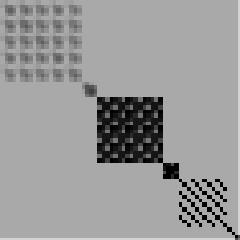
\includegraphics[scale=0.66]{figures/logo.pdf}};
\end{tikzpicture}
\end{center}

\vfill

\begin{abstract}
  Kronecker-factored approximate curvature \citep[KFAC,][]{martens2015optimizing} is arguably one of the most prominent curvature approximations in deep learning.
  Its applications range from optimization to Bayesian deep learning, training data attribution with influence functions, and model compression or merging.
  While the intuition behind KFAC is easy to understand, its implementation is tedious: It comes in many flavours, has common pitfalls when translating the math to code, and is challenging to test, which complicates ensuring a properly functioning implementation.
  Some of the authors themselves have dealt with these challenges and experienced the discomfort of not being able to fully test their code.
  Thanks to recent advances in understanding KFAC, we are now able to provide test cases and a recipe for a reliable KFAC implementation.
  \emph{This tutorial is meant as a ground-up introduction to KFAC.}
  In contrast to the existing work, our focus lies on providing both math and code side-by-side, and providing test cases based on latest insights into KFAC that are scattered throughout the literature.
  We hope this tutorial provides a contemporary view onto KFAC that
  allows beginners to gain a deeper understanding of this curvature approximation, while lowering the barrier to its implementation, extension, and usage in practise.
\end{abstract}

\vfill

\paragraph{Version:} \today\,(v1.0.0)

\paragraph{About the length of this document.}
Before you close this document because of its page number, take a moment to scroll through it.
You will realize that the effective length of this tutorial is much shorter than suggested by its page number.
This is because \emph{we use an experimental two-column layout which presents text and code in parallel} and leads to a good amount of white space.
We deliberately chose this format because it allows to explicitly spell out the math in code.

\paragraph{Follow along in code.} The \LaTeX\,\& Python source code is available at \href{\repourl}{\texttt{github.com/f-dangel/kfac-tutorial}}.
This allows you to run the code as you read:
Clone the repository and follow the installation instructions.
You can then run each snippet from the repository root, for instance by calling \texttt{python kfs/basics/forward\_pass.py}.
If you find typos or have suggestions for improving improving explanations, math, or code, please open issues and pull requests.
In doing so, you are contributing to making this tutorial a valuable reference for newcomers.

\vspace{\baselineskip}
%%% Local Variables:
%%% mode: latex
%%% TeX-master: "../main"
%%% End:

\clearpage

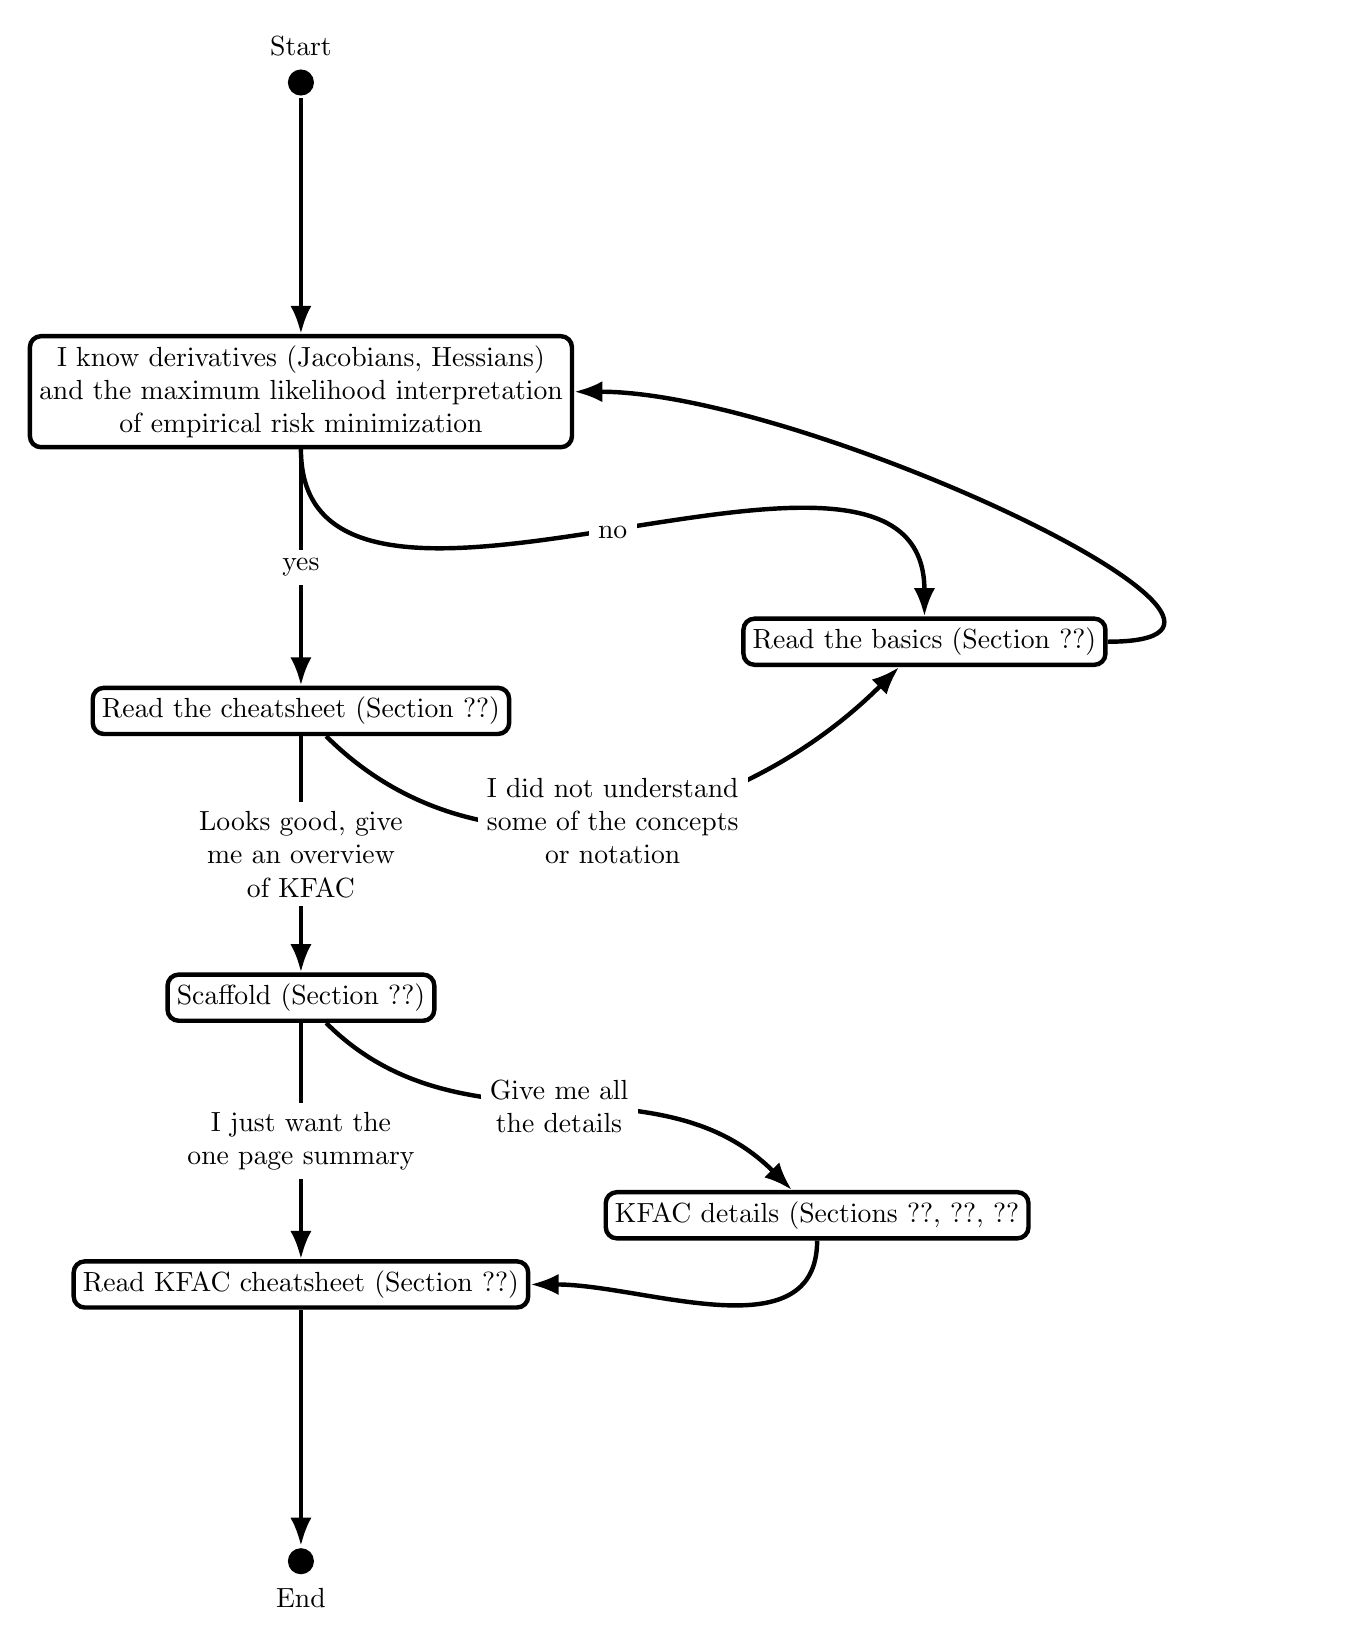
\begin{tikzpicture}[ultra thick, node distance=3cm]
  % define style statement nodes
  \tikzstyle{box} = [rectangle, align=center, minimum height=2.5ex, rounded corners, draw=black]
  \tikzstyle{answer} = [minimum height=2.5ex, fill=white, align=center]

  \node [circle, fill=black] (start) {};
  \node [anchor=south] at (start.north) {Start};

  \node [box, below=of start] (check-basics) {I know derivatives (Jacobians, Hessians)\\ and the maximum likelihood interpretation\\ of empirical risk minimization};
  \draw[-{LaTeX}] (start) -- (check-basics);

  \node [box, below right=of check-basics] (read-basics) {Read the basics (Section ??)};
  \node [box, below=of check-basics] (read-cheatsheet) {Read the cheatsheet (Section ??)};
  \draw[-{LaTeX}] (check-basics) to[out=270, in=90] node [midway, answer] {yes} (read-cheatsheet);
  \draw[-{LaTeX}] (check-basics) to[out=270, in=90] node [midway, answer] {no} (read-basics);
  \draw[-{LaTeX}] (read-basics) to[out=0, in=0] (check-basics);

  \node [box, below=of read-cheatsheet] (scaffold) {Scaffold (Section ??)};
  \draw[-{LaTeX}] (read-cheatsheet) to node [midway, answer] {Looks good, give \\ me an overview\\ of KFAC} (scaffold);
  \draw[-{LaTeX}] (read-cheatsheet) to [out=315, in=225] node [midway, answer] {I did not understand \\ some of the concepts \\ or notation} (read-basics);

  \node[box, below=of scaffold] (kfac-cheatsheet) {Read KFAC cheatsheet (Section ??)};
  \node[box, below right=of scaffold] (kfac-details) {KFAC details (Sections ??, ??, ??};
  \draw[-{LaTeX}] (scaffold) to[out=315, in=135] node [midway, answer] {Give me all \\ the details} (kfac-details);
  \draw[-{LaTeX}] (scaffold) to[out=270, in=90] node [midway, answer] {I just want the \\ one page summary} (kfac-cheatsheet);
  \draw[-{LaTeX}] (kfac-details) to[out=270, in=0] (kfac-cheatsheet);

  \node[circle, fill=black, below=of kfac-cheatsheet] (end) {};
  \node[anchor=north] at (end.south) {End};
  \draw[-{LaTeX}] (kfac-cheatsheet) -- (end);
\end{tikzpicture}
%%% Local Variables:
%%% mode: LaTeX
%%% TeX-master: "../main"
%%% End:

\clearpage

\tableofcontents
\clearpage

\section{Preface}
This is an attempt to bundle scattered knowledge about KFAC into a single document, explain all the technicalities and pitfalls, and present tests to ensure bug-free implementations.

Should answer the following questions:
\begin{itemize}
\item Why do we need this tutorial?
\item Why is this not a Jupyter notebook?
\item What do we gain by explaining KFAC bottom-up?
\item What ML framework do we use and why?
\item What are we \emph{not} doing (e.g.\,building an optimizer)?
\end{itemize}

We use PyTorch~\cite{paszke2019pytorch} and implement everything using \texttt{torch.nn} rather than a functional formulation as we feel that many deep learning practitioners are more familiar with this style.
There could be a JAX or functorch version, too.

\begin{itemize}
\item KFAC approximates the Fisher, which is an outer product of gradients. The gradients involve the output-parameter Jacobian of a weight, which has Kronecker structure,
  \begin{align}
    \jac_{\mW}(\mW \vx) = \vx^{\top} \otimes \mI\,.
  \end{align}
  This implies that the Fisher contains terms of the following form, where $\bullet$ is a placeholder for some matrix,
  \begin{align}
    \left(
    \vx^{\top}\otimes \mI
    \right)^{\top}
    \bullet
    \left(
    \vx^{\top}\otimes \mI
    \right)\,.
  \end{align}

\item The goal is to build up to an abstract general formulation of KFAC.
  Given a compute graph which uses the operations $\vx, \mW \mapsto \mW x$, potentially in multiple places, define a Kronecker approximation of the Fisher.
  Also to show the different degrees of freedom: treating weights \& biases jointly/separately, using reduce versus expand approximation, and treating weight tying, i.e.
  multi-usage of $\mW$.

\end{itemize}
TODO Should mention somewhere that many of the provided examples are already discussed in Felix's PhD thesis~\cite{dangel2023backpropagation}.
%%% Local Variables:
%%% mode: latex
%%% TeX-master: "../main"
%%% End:

\clearpage

\columnratio{0.42}
\begin{paracol}{2}
  \section{Basics}
  \subsection{Empirical risk minimization \& Maximum Likelihood Estimation}

\subsubsection{Deep neural networks}

\subsubsection{Probabilistic interpretation}


\begin{align}
  \gL(\vtheta) &= \sum_{n=1}^N \ell(\vtheta, \vx_n, \vy_n)
  \\
               &=
                 \sum_{n=1}^N c(f(\vtheta, \vx_n), \vy_n)
\end{align}

\switchcolumn[0]

\blindtext

\switchcolumn[1]

\switchcolumn[0]* % sync

\blindtext

\subsection{Derivatives \& Automatic Differentiation}

\begin{caveat}
  In deep learning, we often work with matrices, or higher-dimensional tensors.
  We want to use matrix linear algebra expressions to avoid using heavy index notation.
  This can be achieved by flattening all tensors back into vectors and re-using definitions derivatives from the vector case.
  However, we must be careful when translating the results back to the tensor format, as the translation process depends on the flattening convention.
  Classically, the mathematical derivations prefer a \emph{different} flattening scheme than the one used in deep learning libraries.
\end{caveat}

\switchcolumn[0]*
\subsubsection{Flattening}
There are many ways to flatten the entries of a tensor into a vector.
The two by far most common conventions are (i) last-varies-fastest ($\cvec$) and (ii) first-varies-fastest ($\rvec$).
Their names are easy to remember from their action on a matrix (see \Cref{ex:flattening}): $\cvec$-flattening concatenates columns into a vector (column flattening); $\rvec$-flattening concatenates rows into a vector (row flattening).
Column-flattening is popular in mathematical presentations, while row-flattening is popular in deep learning libraries which lay out tensors in row-major format in memory.
To see their differences, we will implement both.

For arbitrary tensors, we can generalize the matrix flattenings by ordering entries such that either their last index ($\cvec$, \Cref{def:cvec}) or first index ($\rvec$, \Cref{def:rvec}) varies fastest:

\switchcolumn[1]*
\codeblock{basics/flattening}
\switchcolumn[0]

\begin{setup}\label{setup:flattening}
  Let $\tA \in \sR^{N_1 \times \dots \times N_A}$ be a tensor of rank $A$ whose entries are indexed through a tuple $(n_1, \dots, n_A)$ where $n_a \in \{1, \dots, N_a\}$.
\end{setup}
\begin{definition}[$\cvec$, \Cref{flattening}]\label{def:cvec}
  The first-varies-fastest flattening of $\tA$ from \Cref{setup:flattening} is
  \begin{align*}
    \cvec(\tA) =
    \begin{pmatrix}
      \etA_{1,1,\dots,1} \\
      \etA_{2,1,\dots,1} \\
      \vdots \\
      \etA_{N_1,1,\dots,1} \\
      \etA_{1,2,\dots,1} \\
      \vdots \\
      \etA_{N_1,2,\dots,1} \\
      \vdots \\
      \etA_{N_1,N_2,\dots,N_A}
    \end{pmatrix}
    \in \sR ^{N_1 \cdots N_A}\,.
  \end{align*}
\end{definition}

\begin{definition}[$\rvec$, \Cref{flattening}]\label{def:rvec}
  The last-varies-fastest flattening of $\tA$ from \Cref{setup:flattening} is
  \begin{align*}
    \rvec(\tA) =
    \begin{pmatrix}
      \etA_{1,\dots,1,1} \\
      \etA_{1,\dots,1,2} \\
      \vdots \\
      \etA_{1,\dots,1,N_A} \\
      \etA_{1,\dots,2,1} \\
      \vdots \\
      \etA_{1,\dots,2,N_A} \\
      \vdots \\
      \etA_{N_1,\dots,N_{A-1},N_A}
    \end{pmatrix}
    \in \sR ^{N_A \cdots N_1}\,.
  \end{align*}
\end{definition}

In code, we will sometimes require partial flattening of a sub-set of contiguous indices, instead of all indices.
The definitions are analogous, but the flattened indices are surrounded by static ones.

\begin{example}[Matrix flattening, \Cref{flattening}]\label{ex:flattening}
  For a matrix
  \begin{equation*}
    \mA = \begin{pmatrix} 1 & 2 \\ 3 & 4 \end{pmatrix}
  \end{equation*}
  we have
  \begin{equation*}
    \rvec(\mA)
    =
    \begin{pmatrix}
      1 \\ 2 \\ 3 \\ 4
    \end{pmatrix}\,,
    \qquad
    \cvec(\mA)
    =
    \begin{pmatrix}
      1 \\ 3 \\ 2 \\ 4
    \end{pmatrix}\,.
  \end{equation*}
\end{example}
%%% Local Variables:
%%% mode: latex
%%% TeX-master: "../main"
%%% End:


\switchcolumn[0]*
\subsubsection{Jacobians, JVP, VJPs}
Building up to curvature approximations that tackle the approximation of second-order partial derivatives, we start with first-order derivatives.
These are collected into a matrix called the Jacobian, which depends on the flattening convention.
We can multiply with the Jacobian and its transpose via automatic differentiation, without building up the matrix in memory.
These operations are called vector-Jacobian products (VJPs) and Jacobian-vector products (JVPs), respectively.

Machine learning libraries like JAX and PyTorch offer routines for computing Jacobians, VJPs, and JVPs.
However, their interface is functional.
Here, we provide an alternative implementation that accepts nodes of a computation graph rather than functions as input and will be beneficial for modular implementations of neural networks, as we consider later.
We also provide examples for important Jacobians, namely the output-parameter Jacobian of an affine map, \ie a linear layer.
These Jacobians exhibit Kronecker structure, which is the foundation for the `K' in KFAC.
We verify this structure numerically and observe how the flattening convention affects it.

\begin{setup}[Vector-to-vector function]\label{setup:vector_to_vector_function}
  Let function $f: \sR^A \to \sR^B, \va \mapsto \vb = f(\va)$ denote a vector-to-vector function.
\end{setup}

\begin{definition}[Jacobian of a vector-to-vector function]\label{def:vector_jacobian}
  The Jacobian of a vector-to-vector function $f$ from \Cref{setup:vector_to_vector_function}, $\jac_{\va}\vb \in \sR^{B \times A}$, collects the first-order partial derivatives into a matrix such that
  \begin{align*}
    [\jac_{\va} \vb]_{i,j} = \frac{\partial [f(\va)]_i}{\partial [\va]_j}\,.
  \end{align*}
\end{definition}
\Cref{def:vector_jacobian} is limited to vector-to-vector functions.
The more general Jacobian of a tensor-to-tensor function can be indexed with combined indices from the input and output domains:

\begin{setup}[Tensor-to-tensor function]\label{setup:jacobians}
  Consider a tensor-to-tensor function $f: \sR^{A_1 \times \dots \times A_N} \to \sR^{B_1 \times \dots \times B_M}, \tA \mapsto \tB = f(\tA)$ from a rank-$N$ tensor $\tA$ into a rank-$M$ tensor $\tB$.
\end{setup}

\begin{definition}[General Jacobian, \Cref{basics/jacobians}]\label{def:general_jacobian}
  The general Jacobian of $f$ from \Cref{setup:jacobians}, $\tJ_{\tB}\tA$, is a rank-$(M+N)$ tensor that collects the first-order partial derivatives such that
  \begin{align*}
    [\tJ_{\tA}\tB]_{\colored{i_1, \dots, i_M}, \colored[VectorPink]{j_1, \dots, j_N}}
    =
    \frac{\partial [f(\tA)]_{\colored{i_1, \dots, i_M}}}{\partial [\tA]_{\colored[VectorPink]{j_1, \dots, j_N}}}\,.
  \end{align*}
\end{definition}
For $M=N=1$, the general Jacobian reduces to the Jacobian of a vector-to-vector function from \Cref{def:vector_jacobian}.

\switchcolumn[1]*
\codeblock{basics/jacobian_products}
\switchcolumn[0]

\paragraph{Jacobian multiplication.} In practice, this general Jacobian can be prohibitively large and therefore one must almost always work with it in a matrix-free fashion, \ie through VJPs and JVPs.

\begin{definition}[Vector-Jacobian products (VJPs), \Cref{basics/jacobian_products}]\label{def:vjp}
  Given a tensor-to-tensor function $f$ from \Cref{setup:jacobians} and a tensor $\tV \in \sR^{B_1 \times \dots \times B_M}$ in the output domain, the vector-Jacobian product (VJP) $\tU$ of $\tV$ and $\tJ_{\tA}\tB$ lives in $f$'s input domain and follows by contracting the \colored{output indices},
  \begin{align*}
    & [\tU]_{j_1, \dots, j_N}
    \\
    & =
      \colored{\sum_{i_1, \dots, i_M}}
      [\tV]_{\colored{i_1, \dots, i_M}}
      [\tJ_{\tA}\tB]_{\colored{i_1, \dots, i_M}, j_1, \dots, j_N}\,.
  \end{align*}
\end{definition}
For $M=N=1$, $\tV, \tU \to \vv, \vu$ are column vectors, $\tJ_{\tA}\tB \to \jac_{\va}\vb$ is a matrix, and the VJP is $\vu^{\top} = \vv^{\top} (\jac_{\va}\vb)$ or $\vu = (\jac_{\va}\vb)^{\top} \vv$, \ie multiplication with the transpose Jacobian.

VJPs are at the heart of reverse-mode automatic differentiation, aka backpropagation (this is why $\tU$ is often called the \emph{pull-back} or \emph{backpropagation} of $\tV$ through $f$).
Therefore, they are easy to implement with standard functionality (\eg \texttt{autograd.grad} in PyTorch).

The other relevant contraction is between the Jacobian and a vector from the input domain:

\begin{definition}[Jacobian-vector products (JVPs), \Cref{basics/jacobian_products}]\label{def:jvp}
  Given a tensor-to-tensor function $f$ from \Cref{setup:jacobians} and a tensor $\tV \in \sR^{A_1 \times \dots \times A_N}$ in the input domain, the Jacobian-vector product (JVP) $\tU$ between $\tV$ and $\tJ_{\tA}\tB$ lives in $f$'s output domain and follows by contracting the \colored[VectorPink]{input indices},
  \begin{align*}
    & [\tU]_{j_1, \dots, j_M}
    \\
    & =
      \colored[VectorPink]{\sum_{i_1, \dots, i_N}}
      [\tJ_{\tA}\tB]_{j_1, \dots, j_M, \colored[VectorPink]{i_1, \dots, i_N}}
      [\tV]_{\colored[VectorPink]{i_1, \dots, i_N}}\,.
  \end{align*}
\end{definition}
For the vector case, $\tU, \tV, \tJ_{\tA}\tB \to \vu, \vv, \jac_{\va}\vb$, the JVP is $\vu = (\jac_{\va}\vb) \vv$, as suggested by its name.
JVPs are common in forward-mode automatic differentiation ($\tU$ is often called the \emph{pushforward} of $\tV$ through $f$).
Only recently has this mode garnered attention.
The current JVP functionality in ML libraries usually follows a functional API.
To obtain an implementation that accepts variables from a computation graph and is more compatible with the modular approach we chose in this tutorial, we can use a trick that implements a JVP using two VJPs \cite{townsend2017new}.

\switchcolumn[1]*
\begin{figure}[!h]
  \centering
  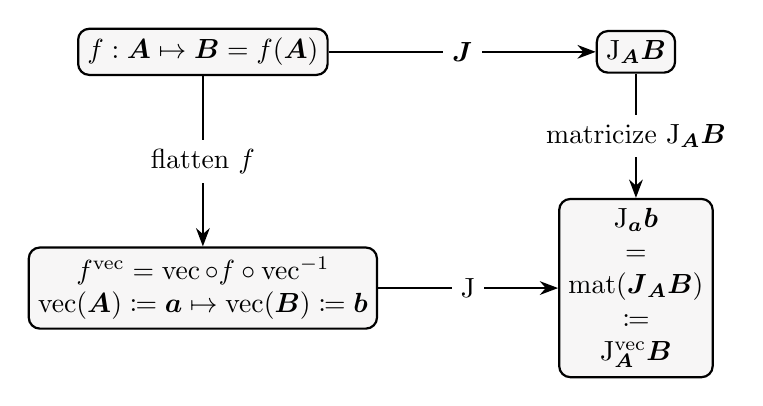
\begin{tikzpicture}[%
    % font=\scriptsize,%
    thick,
    box/.style = {rectangle, draw=black, rounded corners, fill=VectorGray!50},%%
    ]
    \node[box] (A) at (0,0) {$f: \tA \mapsto \tB = f(\tA)$};
    \node[box] (B) at (5.5,0) {$\jac_{\tA}\tB$};
    \node[box, align=center] (C) at (0,-3) {%
      $f^{\vec} = \vec \circ f \circ \vec^{-1}$\\%
      $\vec(\tA) \coloneq \va \mapsto \vec(\tB) \coloneq \vb$%
    };
    \node[box, align=center] (D) at (5.5,-3) {%
      $\jac_{\va} \vb$\\%
      $=$\\%
      $\mat(\tJ_{\tA}\tB)$\\%
      $\coloneq$\\%
      $\jac^{\vec}_{\tA}\tB$%
    };
    \draw[-Stealth] (A.east) -- node[fill=white] {$\tJ$} (B.west);
    \draw[-Stealth] (A.south) -- node[fill=white] {flatten $f$} (C.north);
    \draw[-Stealth] (C.east) -- node[fill=white] {$\jac$} (D.west);
    \draw[-Stealth] (B.south) -- node[fill=white] {matricize $\jac_{\tA}\tB$} (D.north);
  \end{tikzpicture}
  \caption{\textbf{Flattening and taking the Jacobian commute and lead to the same matricized Jacobian.}
    $\vec$ denotes one of the flattening conventions from \Cref{def:cvec,def:rvec}.
    $\mat$ denotes matricization (two partial flattenings for row and column dimensions, respectively).}\label{fig:commutative-diagram-jacobian}
\end{figure}
\switchcolumn[0]

\paragraph{Matricization.}
Jacobian products are efficient, but somewhat abstract to work with, as we cannot `touch' the full tensor.
Often, we would also like to think about this tensor as a matrix to be able to present derivations in linear algebra notation.

We can reduce the general Jacobian tensor back to the Jacobian matrix in two different ways: We can either (i) directly matricize the tensor, or (ii) `flatten' the function $f \to f^{\vec}$ such that it consumes and produces vectors, then compute its Jacobian.
Both ways and their resulting Jacobian matrices depend on the flattening convention we choose.
The following definitions are consistent in the sense that both of the aforementioned approaches yield the same result, illustrated by this commutative diagram in \cref{fig:commutative-diagram-jacobian}.


\switchcolumn[1]
\codeblock{basics/jacobians}
\switchcolumn[0]

For this tutorial, the two matrices of interest are the $\cvec$- and $\rvec$-Jacobians.
The $\cvec$-Jacobian is used in mathematical derivations in the literature.
The $\rvec$-Jacobian is common in code.

\begin{definition}[$\cvec$-Jacobian, \Cref{basics/jacobians}]\label{def:cvec_jacobian}
  For a tensor-to-tensor function $f$ from \Cref{setup:jacobians}, its $\cvec$-Jacobian $\jac^{\cvec}_{\tA}\tB \in \sR^{A_N \cdots A_1 \times B_M \cdots B_1}$ is attained by flattening the input and output tensors with $\cvec$ and applying the Jacobian definition for vectors,
  \begin{align*}
    [\jac^{\cvec}_{\tA}\tB]_{i,j}
    =
    \frac{\partial [\cvec(f(\tA))]_i}{\partial [\cvec(\tA)]_j}\,.
  \end{align*}
\end{definition}

\begin{definition}[$\rvec$-Jacobian, \Cref{basics/jacobians}]\label{def:rvec_jacobian}
  For a tensor-to-tensor function $f$ from \Cref{setup:jacobians}, its $\rvec$-Jacobian $\jac^{\rvec}_{\tA}\tB \in \sR^{A_1 \cdots A_N \times B_1 \cdots B_M}$ is attained by flattening the input and output tensors with $\rvec$ and applying the Jacobian definition for vectors,
  \begin{align*}
    [\jac^{\rvec}_{\tA}\tB]_{i,j}
    =
    \frac{\partial [\rvec(f(\tA))]_i}{\partial [\rvec(\tA)]_j}\,.
  \end{align*}
\end{definition}

\paragraph{Example.} The two Jacobians usually differ from each other, albeit in subtle ways.
We highlight their differences on a linear layer, which will be useful later on when we discuss KFAC (\Cref{ex:linear_layer_jacobians}, numerically verified in \cref{basics/jacobians_linear_layer}).
This example reveals two insights:
\begin{itemize}
\item There is a Kronecker structure in the linear layers' Jacobian \wrt its weight.
  This structure is the foundation for the `K' in KFAC.

\item The order of Kronecker factors is reversed depending on the flattening scheme.
  Therefore, we need to be careful when translating results from one convention to the other.
\end{itemize}

\switchcolumn[1]
\begin{example}[$\cvec$- and $\rvec$-Jacobians of a linear layer \wrt its weights, \Cref{basics/jacobians_linear_layer}]\label{ex:linear_layer_jacobians}
  Consider an affine map with weight matrix $\mW \in \sR^{D_{\text{out}} \times D_{\text{in}}}$, bias vector $\vb \in \sR^{D_{\text{out}}}$, input vector $\vx \in \sR^{D_{\text{in}}}$ and output vector $\vz \in \sR^{D_{\text{out}}}$,
  \begin{align*}
    \vz
    \coloneqq
    \mW \vx + \vb
    =
    \begin{pmatrix}
      \mW & \vb
    \end{pmatrix}
    \begin{pmatrix}
      \vx \\ 1
    \end{pmatrix}
    \coloneqq
    \tilde{\mW}
    \tilde{\vx}\,.
  \end{align*}
  To express this operation as matrix-vector multiplication, we combine weight and bias into a single matrix $\tilde{\mW}$ and augment the input with a one, yielding $\tilde{\vx}$, to account for the bias contribution.

  The linear layer's $\cvec$-Jacobian \wrt the combined weight is
  \begin{align*}
    \jac^{\cvec}_{\tilde{\mW}}\vz
    =
    \tilde{\vx}^{\top}
    \otimes
    \mI_{D_{\text{out}}}\,.
  \end{align*}
  In contrast, the $\rvec$-Jacobian is
  \begin{align*}
    \jac^{\rvec}_{\tilde{\mW}}\vz
    =
    \mI_{D_{\text{out}}}
    \otimes
    \tilde{\vx}^{\top}\,,
  \end{align*}
  see \Cref{basics/jacobians_linear_layer}.
  Note that the order of Kronecker factors is \emph{reversed}, depending on the flattening scheme.
\end{example}
\switchcolumn[0]

\switchcolumn[1]
\codeblock{basics/jacobians_linear_layer}
\switchcolumn[0]


% NOTE This example is about weight sharing, which will not be part of the tutorial's
% first version.
\begin{comment}
  \begin{example}[$\cvec$- and $\rvec$-weight Jacobians of a linear layer with weight sharing]
    Consider the same affine map from above, but now processing multiple input vectors $\mX = \begin{pmatrix}\vx_1 & \dots & \vx_S\end{pmatrix} \in \sR^{D_{\text{in}}\times S}$, yielding a sequence $\mZ = \begin{pmatrix} \vz_1 & \dots & \vz_S\end{pmatrix} \in \sR^{D_{\text{out}}\times S}$ where each $\vz_s$ is produced like above.
    The parameters are \emph{shared} over all vectors in the input sequence.
    In matrix notation,
    \begin{align*}
      \mZ
      & \coloneqq
        \mW \mX + \vb \vone^{\top}_S
      \\
      & =
        \begin{pmatrix}
          \mW & \vb
        \end{pmatrix}
        \begin{pmatrix}
          \mX \\ \vone^{\top}_S
        \end{pmatrix}
        \coloneqq
        \tilde{\mW}
        \tilde{\mX}\,.
    \end{align*}
    The $\cvec$-Jacobian \wrt the combined weight is
    \begin{align*}
      \jac^{\cvec}_{\tilde{\mW}}\mZ
      =
      \tilde{\mX}^{\top}
      \otimes
      \mI_{D_{\text{out}}}\,.
    \end{align*}
    In contrast, the $\rvec$-Jacobian is
    \begin{align*}
      \jac^{\rvec}_{\tilde{\mW}}\mZ
      =
      \mI_{D_{\text{out}}}
      \otimes
      \tilde{\mX}^{\top}\,.
    \end{align*}
  \end{example}

  \switchcolumn[1]
  \codeblock{basics/jacobians_shared_linear_layer}
\end{comment}

%%% Local Variables:
%%% mode: latex
%%% TeX-master: "../main"
%%% End:


\switchcolumn[0]*
\subsubsection{Hessians, HVPs}
Now that we have covered first-order derivatives, let's move on to second-order derivatives and develop the necessary concepts to understand KFAC, as well as their implementation.
Second-order derivatives are collected into an object called \emph{the Hessian}.
For our purposes, it will be sufficient to consider the Hessian of functions producing a scalar-valued output.
Let's start with the definition of the Hessian of a vector-to-scalar function.

\begin{setup}[Vector-to-scalar function]\label{setup:vector_to_scalar_function}
  Let $\vf: \sR^A \to \sR, \va \mapsto b = f(\va)$ be a vector-to-scalar function.
\end{setup}

\begin{definition}[Hessian of a vector-to-scalar function]\label{def:vector_hessian}
  The Hessian of a vector-to-scalar function $f$ from \Cref{setup:vector_to_scalar_function} is a matrix $\hess_{\va}b \in \sR^{A \times A}$ collecting the second-order partial derivatives of $f$ into a matrix with
  \begin{align*}
    [\hess_{\va}b]_{i,j}
     & =
    \frac{\partial^2 b}{\partial [\va]_i \partial [\va]_j}\,.
  \end{align*}
\end{definition}
This definition is limited to functions with vector-valued arguments. The extension to tensor-to-scalar functions is straightforward; however, it yields a tensor that is less convenient to work with in terms of notation:

\begin{setup}[Tensor-to-scalar function]\label{setup:hessians}
  Consider a tensor-to-scalar function $f: \sR^{A_1 \times \dots \times A_N} \to \sR, \tA \mapsto b = f(\tA)$ from a rank-$N$ tensor $\tA$ into a scalar $b$.
\end{setup}

\begin{definition}[General Hessian of a tensor-to-scalar function, \Cref{basics/hessians}]\label{def:general_hessian}
  The general Hessian of $f$ from \Cref{setup:hessians}, $\tH_{\tA}b \in \sR^{A_1 \times \dots \times A_N \times A_1 \times \dots \times A_N}$, collects the second-order partial derivatives of $f$ into a tensor with
  \begin{align*}
     & [\tH_{\tA}b]_{\colored{i_1, \dots, i_N}, \colored[VectorPink]{j_1, \dots, j_N}}
    \\
     & =
    \frac{\partial^2 b}{\partial [\tA]_{\colored{i_1, \dots, i_N}} \partial [\tA]_{\colored[VectorPink]{j_1, \dots, j_N}}}\,.
  \end{align*}
\end{definition}

\switchcolumn[1]*
\codeblock{basics/hessian_product}
\switchcolumn[0]

\paragraph{Hessian multiplication.}
Just like for Jacobians, the Hessian tensor is usually too large to be stored in memory.
Hence, one usually works with it implicitly through matrix-vector products, which can be done without computing the Hessian:

\begin{definition}[Hessian-vector products (HVPs), \Cref{basics/hessian_product}]\label{def:hvp}
  Given a tensor-to-scalar function $f$ from \Cref{setup:hessians} and a tensor $\tV \in \sR^{A_1 \times \dots \times A_N}$ in the input domain, the Hessian-vector product (HVP) $\tU$ of $\tV$ with $\tH_{\tA}b$ is the result of contraction with one of the Hessian's \colored{input indices},
  \begin{align*}
     & [\tU]_{i_1, \dots, i_N}
    \\
     & =
    \colored{\sum_{j_1, \dots, j_N}}
    [\tH_{\tA}b]_{i_1, \dots, i_N, \colored{j_1, \dots, j_N}} [\tV]_{\colored{j_1, \dots, j_N}}\,.
  \end{align*}
\end{definition}
For the vector case $N=1$, we have $\tV, \tA, \tH_{\tA}b \to \vv, \va, \hess_{\va}b$ and $\tU \to \vu = \hess_{\va} b$ as suggested by the name`Hessian-vector product'.

One way to multiply by the Hessian uses the so-called Pearlmutter trick~\cite{pearlmutter1994fast}.
It relies on the fact that multiplication with higher-order derivatives can be done by nested first-order differentiation.
Hence, multiplication with the Hessian can be done with two VJPs (\Cref{basics/hessian_product}).
In fact, this snippet implements a slightly more general Hessian that can handle differentiating twice \wrt \emph{different}, in contrast to the same, arguments.
It is not essential for understanding KFAC, and we will only use it to visualize curvature matrices in \Cref{subsec:curvature-matrices}.
In the context of KFAC, we do not care about these mixed second-order derivatives.

\switchcolumn[1]
\begin{figure}[!h]
  \centering
  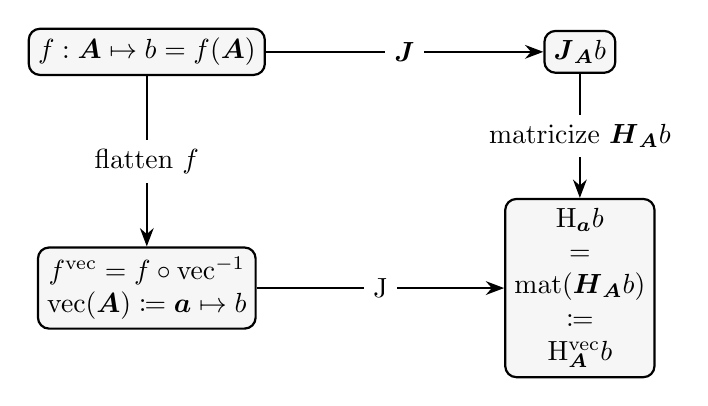
\begin{tikzpicture}[%
      % font=\scriptsize,%
      thick,
      box/.style = {rectangle, draw=black, rounded corners, fill=VectorGray!50},%%
    ]
    \node[box] (A) at (0,0) {$f: \tA \mapsto b = f(\tA)$};
    \node[box] (B) at (5.5,0) {$\tJ_{\tA}b$};
    \node[box, align=center] (C) at (0,-3) {%
      $f^{\vec} = f \circ \vec^{-1}$\\%
      $\vec(\tA) \coloneq \va \mapsto b$%
    };
    \node[box, align=center] (D) at (5.5,-3) {%
      $\hess_{\va} b$\\%
      $=$\\%
      $\mat(\tH_{\tA}b)$\\%
      $\coloneq$\\%
      $\hess^{\vec}_{\tA}b$%
    };
    \draw[-Stealth] (A.east) -- node[fill=white] {$\tJ$} (B.west);
    \draw[-Stealth] (A.south) -- node[fill=white] {flatten $f$} (C.north);
    \draw[-Stealth] (C.east) -- node[fill=white] {$\jac$} (D.west);
    \draw[-Stealth] (B.south) -- node[fill=white] {matricize $\tH_{\tA}b$} (D.north);
  \end{tikzpicture}
  \caption{\textbf{Flattening and taking the Hessian commute and lead to the same matricized Hessian.}
    $\vec$ denotes one of the flattening conventions from \Cref{def:cvec,def:rvec}.
    $\mat$ denotes matricization and involves two partial flattenings for row and column dimensions.}\label{fig:commutative-diagram-hessian}
\end{figure}
\switchcolumn[0]

\paragraph{Matricization:} For notational convenience, we will also define matricized versions of the general Hessian from \Cref{def:general_hessian}; the $\cvec$-, and $\rvec$-Hessian. Just like for the Jacobians, it does not matter whether we first flatten the function's input space then compute the Hessian, or compute the general Hessian then matricize it (\Cref{fig:commutative-diagram-hessian}).
The following definitions are consistent for both ways.

\switchcolumn[1]
\codeblock{basics/hessians}
\switchcolumn[0]

\begin{definition}[$\cvec$-Hessian, \Cref{basics/hessians}]\label{def:cvec_hessian}
  For a tensor-to-scalar function $f$ from \Cref{setup:hessians}, the $\cvec$-Hessian $\hess_{\tA}^{\cvec}b \in \sR^{A_N \cdots A_1 \times A_N \cdots A_1}$ results from flattening the input tensor with $\cvec$ and applying the Hessian from \Cref{def:vector_hessian},
  \begin{align*}
    [\hess^{\cvec}_{\tA}b]_{i, j}
     & =
    \frac{\partial^2 b}{\partial [\cvec(\tA)]_{i} \partial [\cvec(\tA)]_{j}}\,.
  \end{align*}
\end{definition}

\begin{definition}[$\rvec$-Hessian, \Cref{basics/hessians}]\label{def:rvec_hessian}
  For a tensor-to-scalar function $f$ from \Cref{setup:hessians}, the $\rvec$-Hessian $\hess_{\tA}^{\rvec}b \in \sR^{A_1 \cdots A_N \times A_1 \cdots A_N}$ results from flattening the input tensor with $\rvec$ and applying the Hessian from \Cref{def:vector_hessian},
  \begin{align*}
    [\hess^{\rvec}_{\tA}b]_{i, j}
     & =
    \frac{\partial^2 b}{\partial [\rvec(\tA)]_{i} \partial [\rvec(\tA)]_{j}}\,.
  \end{align*}
\end{definition}

Whenever we consider vector-to-scalar functions, both Hessians are identical, and we thus suppress the flattening scheme and write $\hess_{\va}b$.

\paragraph{Examples.}
Let's look at important Hessian examples we will return to later in the text.
We can use them to verify our Hessian implementation.

\switchcolumn[1]
\codeblock{basics/hessian_ce_loss}
\switchcolumn[0]

\begin{example}[Softmax cross-entropy loss Hessian, \Cref{basics/hessian_ce_loss}]\label{ex:hessian-crossentropyloss}
  Consider the softmax cross-entropy loss function between the vector-valued logits $\vf \in \sR^C$ and a class label $y \in \{1, \dots, C\}$ from \Cref{ex:cross_entropy_loss}:
  \begin{align*}
    c(\vf, y)
     & =
    -\log([\vsigma(\vf)]_y)\,.
  \end{align*}
  with $\vsigma(\vf) = \softmax(\vf) \in \sR^C$.
  Its Hessian \wrt $\vf$ is diagonal-minus-rank-one,
  \begin{align*}
    \hess_{\vf} c(\vf, y)
    =
    \diag(\vsigma) - \vsigma \vsigma^\top\,.
  \end{align*}
  See \eg~\citet{dangel2020modular} for a derivation.
\end{example}

\switchcolumn[1]
\codeblock{basics/hessian_mse_loss}

\switchcolumn[0]
\begin{example}[Square loss Hessian, \Cref{basics/hessian_mse_loss}]\label{ex:square_loss_hessian}
  Consider the square loss function between a vector-valued input $\vf \in \sR^C$ and its associated target $\vy \in \sR^C$ from \Cref{ex:square_loss}:
  \begin{align*}
    c(\vf, \vy)
     & =
    \frac{1}{2}\left\lVert
    \vf - \vy
    \right\rVert^2
    \\
     & =
    \frac{1}{2}(\vf - \vy)^{\top} \mI (\vf - \vy)\,.
  \end{align*}
  Its Hessian \wrt $\vf$ is the identity,
  \begin{align*}
    \hess_{\vf} \ell(\vf, \vy)
    =
    \mI_C\,.
  \end{align*}
\end{example}

%%% Local Variables:
%%% mode: latex
%%% TeX-master: "../main"
%%% End:


\switchcolumn[0]*
\subsection{Curvature Matrices in Deep Learning}
\subsubsection{The Hessian}

\subsubsection{The Generalized Gauss-Newton (GGN)}
Linearization
\subsubsection{The Fisher}
Probabilistic perspective

Explain type-1 versus type-2
\subsubsection{The Connection between GGN \& Fisher}
\subsubsection{The Empirical Fisher (EF)}

%%% Local Variables:
%%% mode: latex
%%% TeX-master: "../main"
%%% End:


  \switchcolumn[0]*
\end{paracol}

\clearpage
\begin{paracol}{1}
  \section{Cheatsheet: Basics}
  \begin{itemize}
\item Risk minimization and tractable empirical risk minimization (\Cref{subsec:empirical-risk-minimization})
  \begin{align*}
    \argmin_{\vtheta} \gL_{p_{\text{data}}(\rvx, \rvy)}(\vtheta)
    \qquad
    &\text{where}\qquad
      \gL_{p_{\text{data}}(\rvx, \rvy)}(\vtheta) \coloneq \E_{(\vx, \vy) \sim p_{\text{data}}(\rvx, \rvy)}
      \left[
      c(f(\vx, \vtheta), \vy)
      \right]
    &\text{(intractable)}
      \shortintertext{(use empirical density $p_{\sD}(\rvx, \rvy) = \frac{1}{N} \sum_n \delta(\rvx - \vx_n) \delta(\rvy - \vy_n)$ from data $\sD = \{ (\vx_n, \vy_n) \sim p_{\text{data}} \mid n=1, \dots, N \}$)}
      \argmin_{\vtheta} \gL_{\sD}(\vtheta)
      \qquad
    &\text{where}\qquad
      \gL_{\sD}(\vtheta) \coloneq R \sum_{n=1}^N c(f(\vx_n; \vtheta), \vy_n)\,.
    &\text{(tractable)}
  \end{align*}
  (changing the reduction factor $R$ does not change the optimization problem's solution)

\item Common criterion functions and their reduction constants (\Cref{ex:square_loss,ex:cross_entropy_loss})
  \begin{align*}
    &\begin{matrix}
      \text{Square loss}
      \\
      \text{(\texttt{MSELoss})}
    \end{matrix}
      \qquad
    &c(\vf, \vy) = \frac{1}{2} \left\lVert \vf - \vy \right\rVert_2^2\,,
      \qquad
    &R =
      \begin{cases}
        2 & \text{\texttt{reduction="sum"}} \\
        \frac{2}{N \dim(\vy)} & \text{\texttt{reduction="mean"}}
      \end{cases}
    \\
    &\begin{matrix}
      \text{Softmax cross-entropy loss}\\
      \text{(\texttt{CrossEntropyLoss})}
    \end{matrix}
      \qquad
    &c(\vf, y) = - \log( [\softmax(\vf)]_y)\,,
      \qquad
    &R =
      \begin{cases}
        1 & \text{\texttt{reduction="sum"}} \\
        \frac{1}{N \dim(\vf)} & \text{\texttt{reduction="mean"}}
      \end{cases}
  \end{align*}

\item Probabilistic interpretation of a neural net: Parameterize $p(\rvx, \rvy \mid \vtheta) = p_{\text{data}}(\rvx) p(\rvy \mid \rvx, \vtheta) = p_{\text{data}}(\rvx) r(\rvy \mid f(\rvx, \vtheta))$
  \begin{align*}
    \argmin_{\vtheta} \mathrm{KL}( p_{\text{data}}(\rvx, \rvy) \mid\mid p(\rvx, \rvy \mid \vtheta) )
    \quad\Leftrightarrow\quad
    &\argmin_{\vtheta} \E_{p_{\text{data}}(\rvx)} \E_{r(\rvy \mid \rvx, \vtheta)} \left[
      - \log r(\rvy \mid f(\rvx, \vtheta))
      \right]
    &\text{(intractable)}
      \shortintertext{(use empirical density to make tractable)}
      \qquad
    &\argmin_{\vtheta} - R \sum_{n=1}^N \log r(\rvy=\vy_n \mid f(\rvx=\vx_n, \vtheta))
    &\text{(tractable)}
  \end{align*}

\item Common criteria are negative log-likelihoods: $c(\vf, \vy) = - \log r(\rvy=\vy \mid f(\rvx, \vtheta) = \vf)$ (\Cref{ex:square_loss_probabilistic,ex:cross_entropy_loss_probabilistic})
  \begin{align*}
    &\text{Square loss (\texttt{MSELoss})}
      \qquad
    &r(\rvy \mid \vf) = \gN( \rvy \mid \vmu = \vf, \mSigma = \mI)
    \\
    &\text{Softmax cross-entropy loss (\texttt{CrossEntropyLoss})}
      \qquad
    &r(\ry \mid \vf) = \gC( \ry \mid \vsigma = \softmax(\vf))
  \end{align*}

\item Shorthands: Per-datum prediction $\vf_n(\vtheta) = f(\vx_n, \vtheta)$, criterion $c_n(\vf_n) = c(\vf_n, \vy_n)$, and loss $\ell_n(\vtheta) = c_n(\vf_n(\vtheta))  $

\item Net Jacobian $\jac_{\vtheta}\vf \in \sR^{\dim(\gF) \times D}$, $[\jac_{\vtheta} \vf]_{i,j} = \frac{\partial [\vf]_i}{\partial [\vtheta]_j}$, criterion Hessian $\hess_{\vf} c \in \sR^{\dim(\gF) \times \dim(\gF)}$, $[\hess_{\vf}c]_{i,j} = \frac{\partial^2 c}{\partial [\vf]_i \partial [\vf]_j}$

\item Hessian, generalized Gauss-Newton, type-II/I/empirical Fishers ($\vf_n \coloneq f(\vx_n, \vtheta)$, $\rvf = f(\rvx, \vtheta)$, $\tilde{\vy}_{n,m} \sim r(\rvy \mid \rvf = \vf_n)$)
  \begin{align*}
    \hess_{\vtheta} \gL(\vtheta)
    &= R \sum_{n=1}^N \hess_{\vtheta} c(\vf_n, \vy_n)
      = -R \sum_{n=1}^N \hess_{\vtheta} \log r(\rvy = \vy_n \mid \rvf = \vf_n)
    \\
    \mG(\vtheta)
    &= R \sum_{n=1}^N
      \jac_{\vtheta} \vf_n^{\top}
      \left(
      \hess_{\vf_n} c(\vf_n, \vy_n)
      \right)
      \jac_{\vtheta} \vf_n
      =
      R \sum_{n=1}^N
      \jac_{\vtheta} \vf_n^{\top}
      \left(
      -\hess_{\vf_n} \log r(\rvy = \vy_n \mid \rvf = \vf_n)
      \right)
      \jac_{\vtheta} \vf_n
    \\
    \mF^{\text{II}}(\vtheta)
    &=
      \lim_{M \to \infty}
      \frac{R}{M}
      \sum_{n=1}^N
      \jac_{\vtheta} \vf_n^{\top}
      \left[
      \hess_{\vf_n}(\underbrace{- \log r(\rvy = \tilde{\vy}_{n,m} \mid \rvf = \vf_n)}_{= c(\vf_n, \tilde{\vy}_{n,m})} )
      \right]
      \jac_{\vtheta} \vf_n
    \\
    \mF^{\text{I}}(\vtheta)
    &=
      \lim_{M \to \infty}
      \frac{R}{M}
      \sum_{n=1}^N
      \jac_{\vtheta} \vf_n^{\top}
      \left[
      -\nabla_{\vf_n} \log r(\rvy = \tilde{\vy}_{n,m} \mid \rvf = \vf_n)
      (-\nabla_{\vf_n} \log r(\rvy = \tilde{\vy}_{n,m} \mid \rvf = \vf_n))^{\top}
      \right]
      \jac_{\vtheta} \vf_n
    \\
    \mE(\vtheta)
    &=
      R
      \sum_{n=1}^N
      (\nabla_{\vtheta} c(\vf_n, \vy_n))
      (\nabla_{\vtheta} c(\vf_n, \vy_n))^{\top}
  \end{align*}
  \begin{itemize}
  \item In expectation notation (coloured parts coincide for the above criterion functions, hence GGN = Fisher)
    \begin{align*}
      \hess_{\vtheta} \gL_{\sD}(\vtheta)
      &\propto
        \E_{p_{\sD}(\rvx)}
        \E_{p_{\sD}(\rvy \mid \rvx)}
        \left[
        -\hess_{\vtheta} \log r(\rvy \mid \rvf)
        \right]
      \\
      \mF(\vtheta)
      &\propto
        \E_{p_{\sD}(\rvx)}
        \E_{r(\rvy \mid \rvf)}
        \left[
        -\hess_{\vtheta} \log r(\rvy \mid \rvf)
        \right]
      \\
      \mG(\vtheta)
      &\propto
        \E_{p_{\sD}(\rvx)}
        \left[
        \jac_{\vtheta} \rvf^{\top}
        \textcolor{VectorBlue}{
        \E_{p_{\sD}(\rvy \mid \rvx)}
        \left[
        -\hess_{\rvf} \log r(\rvy \mid \rvf)
        \right]
        }
        \jac_{\vtheta} \rvf
        \right]
      \\
      \mF^{\text{II}}(\vtheta)
      &\propto
        \E_{p_{\sD}(\rvx)}
        \left[
        \jac_{\vtheta} \rvf^{\top}
        \textcolor{VectorBlue}{
        \E_{r(\rvy \mid \rvf)}
        \left[
        -\hess_{\rvf} \log r(\rvy \mid \rvf)
        \right]
        }
        \jac_{\vtheta} \rvf
        \right]
      \\
      \mF^{\text{I}}(\vtheta)
      &\propto
        \E_{p_{\sD}(\rvx)}
        \left[
        \jac_{\vtheta} \rvf^{\top}
        \textcolor{VectorBlue}{
        \E_{r(\rvy \mid \rvf)}
        \left[
        -\nabla_{\rvf} \log r(\rvy \mid \rvf)
        (
        -\nabla_{\rvf} \log r(\rvy \mid \rvf)
        )^{\top}
        \right]
        }
        \jac_{\vtheta} \rvf
        \right]
      \\
      \mE(\vtheta)
      &\propto
        \E_{p_{\sD}(\rvx)}
        \left[
        \jac_{\vtheta} \rvf^{\top}
        \E_{p_{\sD}(\rvy \mid \rvx)}
        \left[
        -\nabla_{\rvf} \log r(\rvy \mid \rvf)
        (
        -\nabla_{\rvf} \log r(\rvy \mid \rvf)
        )^{\top}
        \right]
        \jac_{\vtheta} \rvf
        \right]
    \end{align*}
  \end{itemize}
\item Gradients (\Cref{ex:square-loss-gradient,ex:cross-entropy-loss-gradient}), Hessians (\Cref{ex:hessian-crossentropyloss,ex:square_loss_hessian}), and symmetric Hessian decompositions (\Cref{ex:mseloss_hessian_factorization,ex:crossentropyloss_hessian_factorization}) of criterion functions
  \begin{align*}
    &
      \qquad&\nabla_{\vf} c(\vf, \vy)
              \qquad&\hess_{\vf} c(\vf, \vy)
                      \qquad&\mS,\, \mS \mS^{\top} = \hess_{\vf} c(\vf, \vy)
    \\
    &
      \begin{matrix}
        \text{Square loss}\\
        \text{(\texttt{MSELoss})}
      \end{matrix}
    & \vf - \vy
      \qquad& \mI
              \qquad& \mI
    \\
    &
      \begin{matrix}
        \text{Softmax cross-entropy loss}\\
        (\text{\texttt{CrossEntropyLoss}})\\
        (\vsigma = \softmax(\vf))
      \end{matrix}
      \qquad& \vsigma - \onehot(y)
              \qquad& \diag(\vsigma) - \vsigma \vsigma^{\top}
                      \qquad& \diag(\sqrt{\vsigma}) - \vsigma \sqrt{\vsigma}^{\top}
  \end{align*}
\end{itemize}
%%% Local Variables:
%%% mode: latex
%%% TeX-master: "../main"
%%% End:

\end{paracol}
\clearpage

\begin{paracol}{2}
  \section{KFAC---An Overview}
  \switchcolumn[1]*
\codeblock{kfac/scaffold}
\switchcolumn[0]

KFAC has many nuances that complicate its understanding.
However, we can break down its structure into a general scaffold that simplifies its complexity into manageable sub-tasks (\Cref{kfac/scaffold}).
Here, we discuss the components.

\paragraph{Outline.} At its core, KFAC approximates curvature matrices using Kronecker products, significantly reducing computational and memory costs.
In this section, we start from the general form of relevant curvature matrices, discuss how their structure enables a Kronecker-factored approximation, and introduce the core components of KFAC.
This scaffold---accompanied by the code snippets on the right---serves as the foundation for a systematic implementation, offering intuition on how Kronecker factors are computed and why such a decomposition is beneficial.
We keep the discussion general and highlight how to adapt the code to approximate any curvature matrix introduced in the previous section.
The next section (\Cref{sec:kfac-expand-linear}) will focus on the specific case of KFAC for the generalized Gauss-Newton (GGN) of linear layers.

\paragraph{Curvature matrix structure.} Many relevant matrices---like the GGN, the type-I, type-II, and empirical Fisher---share a common structure
\begin{align}\label{eq:common-structure}
  \begin{split}
    \!\!\mC&(\vtheta^{(i)}) \\
           &= R \sum_n
             (\jac_{\vtheta^{(i)}} \vf_n)^{\top}
             \left[ \bullet(\vf_n, \vy_n) \right]
             (\jac_{\vtheta^{(i)}} \vf_n)\,
  \end{split}
\end{align}
where $\bullet \in \sR^{\dim(\gF) \times \dim(\gF)}$ is a positive semi-definite matrix in the prediction space that depends on the prediction $\vf_n$ and target $\vy_n$.
This term is sandwiched between the Jacobians of the network's prediction with respect to the parameters $\vtheta^{(i)}$ in layer $i$.
Directly computing and storing these matrices is usually intractable, which motivates approximation schemes such as KFAC.
\paragraph{Key idea.} The idea behind KFAC is to exploit a Kronecker-product structure in the Jacobians $\jac_{\vtheta^{(i)}}\vf_n$ to approximate
\begin{align*}
  \mC(\vtheta^{(i)})
  \approx
  \kfac(\mC(\vtheta^{(i)}))
  \coloneqq \mA^{(i)} \otimes \mB^{(i)}.
\end{align*}
For a composition of functions $$f \coloneqq f^{(L)} \circ f^{(L-1)} \circ \dots \circ f^{(1)}$$ with parameters $$\vtheta = \left[ \vtheta^{(1)}, \dots, \vtheta^{(L)} \right],$$ KFAC yields a block-diagonal approximation of the full curvature matrix $\mC(\vtheta)$, where each block corresponds to a layer and is of the form $\kfac(\mC(\vtheta^{(i)})) = \mA^{{(i)}} \otimes \mB^{(i)}$.

In this approximation, $\mA^{(i)}$ is computed from the inputs to layer $i$, and we refer to it as \emph{input-based Kronecker factor}.
Similarly, $\mB^{(i)}$ is computed from gradients \wrt layer $i$'s output, and we call it the \emph{grad-output-based Kronecker factor}.

\subsection{Why use a Kronecker structure?}
Having a Kronecker approximation for $\mC(\vtheta^{(i)})$ has multiple advantages and motivations that coincide well with the block diagonal structure.

\subsubsection{Kronecker Products Are Computationally Efficient}
\label{sec:mem_comp_eff_kron}
Instead of working with the dense representation
\begin{align*} \mA \otimes& \mB  \in \R^{n_1m_1 \times n_2m_2} \\
                          &=\begin{bmatrix}
                            a_{1,1} & \dots & a_{1,n_2} \\
                            \vdots & \ddots & \vdots \\
                            a_{n_1,1} & \dots & a_{n_1,n_2}
                          \end{bmatrix}
  \\
                          &\otimes
                            \begin{bmatrix}
                              b_{1,1} & \dots & b_{1,m_2} \\
                              \vdots & \ddots & \vdots \\
                              b_{m_1,1} &  \dots & b_{m_1,m_2}
                            \end{bmatrix} \\
                          &=\begin{bmatrix}
                            a_{1,1} \mB & \dots & a_{1,n_2} \mB \\
                            \vdots & \ddots & \vdots \\
                            a_{n_1,1} \mB & \dots & a_{n_1,n_2} \mB
                          \end{bmatrix}\,,
\end{align*}
we can express many operations with the Kronecker factors $\mA \in \sR^{n_1 \times n_2}$ and $\mB \in \sR^{m_1 \times m_2}$.
This drastically reduces memory, as we only need to store and handle these smaller matrices (\ie, $\mathcal{O}(n_1n_2 + m_1m_2)$) rather than the full Kronecker product (\ie $\mathcal{O}(n_1n_2m_1m_2)$).
Examples are:

\paragraph{Matrix-vector products.}
Let $\vv \in \R^{n_2m_2}$, then
$$ (\mA \otimes \mB) \vv = \cvec(\mB \mV \mA^{\top}) $$
with $\mV = \cvec^{-1}(\vv) \in \R^{n_2\times m_2}$.
Similarly,
$$ (\mA \otimes \mB) \vv = \rvec(\mA \mV \mB^{\top}) $$
with $\mV = \rvec^{-1}(\vv) \in \R^{m_2\times n_2}$.

\paragraph{Matrix transpose.} $(\mA \otimes \mB)^{\top} = \mA^{\top} \otimes \mB^{\top}$.

\paragraph{Matrix inverse.} $(\mA \otimes \mB)^{-1} = \mA^{-1} \otimes \mB^{-1}$ (assuming the Kronecker factors are invertible).

\paragraph{Matrix multiplication.}
Let $\mC \in \R^{n_2 \times d_1}$ and $\mD \in \R^{m_2 \times d_2}$, then we have
$$ (\mA \otimes \mB)(\mC \otimes \mD) = \mA \mC \otimes \mB \mD\,, $$ \ie we can multiply the Kronecker factors.

\subsubsection{Kronecker Products Naturally Emerge in Curvature Matrices}

Kronecker structure arises naturally in the expression for $\mC(\vtheta^{(i)})$ due to the structure of the layer Jacobians, providing a strong motivation for its use.
To see this, we rewrite $\mC(\vtheta^{(i)})$ from \Cref{eq:common-structure}.

\paragraph{Factorizing the loss Hessian.}
Since $\bullet(\vf_n, \vy_n)$ is a positive semi-definite matrix, it can be decomposed as a sum of outer products of at most $\dim(\gF)$ vectors: $$\bullet(\vf_n, \vy_n) = \sum_{c=1}^{\dim(\gF)} \blacktriangle_c(\vf_n, \vy_n) (\blacktriangle_c(\vf_n, \vy_n))^{\top}$$
where we define $\blacktriangle_{n,c} := \blacktriangle_c(\vf_n, \vy_n) \in \sR^{\dim(\gF)}$ as a vector we will specify later.
Substituting this into \Cref{eq:common-structure}, we obtain
\begin{align*}
  \mC(&\vtheta^{(i)}) \\
  =&
     R \sum_n \sum_{c}
     (\jac_{\vtheta^{(i)}} \vf_n)^{\top}
     \blacktriangle_{n,c} \blacktriangle_{n,c}^{\top}
     (\jac_{\vtheta^{(i)}} \vf_n)\,.
\end{align*}

\paragraph{Separate the layer's Jacobian.}
By applying the chain rule to split the Jacobian at the layer output $\vx^{(i)} = f^{(i)}(\vx^{(i-1)}, \vtheta^{(i)})$, we get
\begin{align*}
  (\jac_{\vtheta^{(i)}} \vf_n)^{\top}
  =
  (\jac_{\vtheta^{(i)}} \vx^{(i)}_n)^{\top}
  (\jac_{\vx_n^{(i)}} \vf_n)^{\top}.
\end{align*}
Substituting this back, the curvature matrix is
\begin{align*}
  \mC(\vtheta&^{(i)}) \\ =& R \sum_n \sum_{c}
                          &&(\jac_{\vtheta^{(i)}} \vx^{(i)}_n)^{\top} \\
             & &&(\jac_{\vx_n^{(i)}} \vf_n)^{\top}
                  \blacktriangle_{n,c}
                  \blacktriangle_{n,c}^{\top}
                  (\jac_{\vx_n^{(i)}} \vf_n) \\
             & &&(\jac_{\vtheta^{(i)}} \vx^{(i)}_n).
\end{align*}

\switchcolumn[1]*
\begin{example}[Curvature matrix of a linear layer as sum of Kronecker products]\label{ex:curvature-matrix-sum-of-kronecker-products}
  Let's illustrate the statement that the curvature matrix becomes a sum of Kronecker products, where one factor stems from the layers Jacobian and one from a backpropagated vector, for a linear layer with weight matrix $\mW$, and using $\cvec$ flattening.
  Let's define the shorthand $\vg_{n,c} \coloneqq (\jac_{\vx_n^{(i)}} \vf_n)^{\top} \blacktriangle_{n,c}$.
  Then, inserting the layer's Jacobian from \Cref{ex:linear_layer_jacobians}, we get
  \begin{align*}
      \mC^{(i)}(\cvec \mW)
      &= 
      R \sum_n \sum_c
      \left(
      {\vx_n^{(i)}}^{\top}\!\!\! \otimes \mI
      \right)^\top
      \!\!\!\vg_{n,c}
      \vg_{n,c}^\top
      \left(
      {\vx_n^{(i)}}^{\top} \!\!\!\otimes \mI
      \right)
      \\
      &=
      R \sum_n \sum_c
      \left(
      \vx_n^{(i)} \otimes \vg_{n,c}
      \right)
      \left(
      {\vx_n^{(i)}}^\top \otimes \vg_{n,c}^\top
      \right)
      \\
      &=
      R \sum_n \sum_c
      \vx_n^{(i)} {\vx_n^{(i)}}^\top
      \otimes
      \vg_{n,c} \vg_{n,c}^\top\,
  \end{align*}
  simply by using the Kronecker product's properties from \Cref{sec:mem_comp_eff_kron}.
  This illustrates that the exact curvature matrix indeed becomes a sum of Kronecker products.
\end{example}
\switchcolumn[0]

\paragraph{Insert the layer's Jacobian.}
The Kronecker structure emerges naturally in the output-parameter Jacobian $\smash{\jac_{\vtheta^{(i)}} \vx_n^{(i)}}$ of a layer.
We saw this in previous chapters for a linear layer (\Cref{ex:linear_layer_jacobians}), whose Jacobian is a Kronecker product of the layer input $\smash{\vx^{(i-1)}_n}$ and an identity matrix.
Inserting the Jacobian, this reduces the \emph{exact} form of $\mC^{(i)}$ to a sum of Kronecker products (fully worked out in \Cref{ex:curvature-matrix-sum-of-kronecker-products}),
\begin{align*}
  \mC^{(i)} = R \sum_n \sum_c \va_n \va_n^{\top} \otimes \vb_{n,c} \vb_{n,c}^{\top}
\end{align*}
where $\va_n$ stems from the layer's Jacobian, \ie the layer's input, and $\vb_{n,c}$ stems from the vector $\blacktriangle_{n,c}$ that is backpropagated to the layer's output by applying the Jacobian $(\jac_{\vx_n^{(i)}} \vf_n)^{\top}$.

Our remaining steps are (i) to specify what $\va_n$ and $\vb_{n,c}$ are, which will depend on the curvature matrix we want to approximate (\Cref{subsec:backpropagated-vectors}), and (ii) how to approximate the sum of Kronecker products as a single Kronecker product (KFAC's expectation approximation, \Cref{def:kfac_exp_approx}).

\switchcolumn[1]*
\codeblock{kfac/backpropagated_vectors}
\switchcolumn[0]

\subsubsection{Kronecker Factor Dependencies}

For the scaffold in \Cref{kfac/scaffold}, let's quickly think about the dependencies of the Kronecker matrices in the above expression.
KFAC results in two distinct Kronecker factors: one based on layer inputs (input-based Kronecker factor $\mA^{(i)}$) and the other based on gradients with respect to the layer output (grad-output-based Kronecker factor $\mB^{(i)}$).
As we will see, we can interpret $(\jac_{\vtheta^{(i)}} \vx_n^{(i)})^{\top} \blacktriangle_{n,c}$ as a \emph{pseudo-gradient}.
In fact, setting
$$\blacktriangle_{n,c} \leftarrow \nabla_{\vf_n} c(\vf_n, \vy_n)\,$$
we obtain
$$(\jac_{\vtheta^{(i)}} \vx_n^{(i)})^{\top} \blacktriangle_{n,c} = \nabla_{\vx_n^{(i)}} c(\vf_n, \vy_n),$$
which is the per-datum loss gradient with respect to layer $i$'s output.
In summary, we identify the following dependencies of the Kronecker factors $\mA^{(i)}$ and $\mB^{(i)}$, justifying their names:
\begin{align*}
  \mA^{(i)} &\text{\quad depends on \quad} \{\vx_{n}^{(i-1)}\}_n \,,
  \\
  \mB^{(i)} &\text{\quad depends on \quad} \{ (\jac_{\vx_n^{(i)}}\vf_{n})^{\top} \blacktriangle_{n,c}\}_{n,c}\,.
\end{align*}

\subsection{Algorithmic Outline}

We now know enough to discuss the scaffold from \Cref{kfac/scaffold}.

\paragraph{Step 1:} Perform a forward pass to compute $\{\vf_n\}_n $, storing the layer inputs $\{\vx_n^{(i-1)} \}_n$ and outputs $\{\vx_n^{(i)}\}_n$ of all layers $i$ whose parameter curvature matrix we want to approximate with KFAC.

\paragraph{Step 2:} Compute the input-based Kronecker factors $\mA^{(i)}$ using the layer inputs $\{\vx_n^{(i-1)}\}_n$.
The details of that will depend on the layer type, and we still have to specify them in later chapters.

\paragraph{Step 3:} Generate the vectors $\{\blacktriangle_{n,c}\}_{n,c}$ to be backpropagated, and backpropagate them to the layer outputs to get the pseudo-gradients $\{(\jac_{\vx_n^{(i)}} \vf_n)^{\top} \blacktriangle_{n,c} \}_{n,c}$.
This step depends on the loss function we are using, and the curvature matrix we want to approximate (\Cref{subsec:backpropagated-vectors}).
Finally, compute the output-based Kronecker factors $\mB^{(i)}$.
The details will again depend on the layer type, and we will specify them in later chapters.

\paragraph{Step 4:} Account for scaling caused by the loss function's reduction $R$.

\paragraph{Step 5:} Return the KFAC approximation in the form $\mA^{(i)}, \mB^{(i)}$ for all supported $i$.

In summary, the scaffold disentangles the task of computing KFAC into three components: (i) computing the input-based Kronecker factors, (ii) generating and backpropagating the vectors $\blacktriangle_{n,c}$, and (iii) computing the grad-output-based Kronecker factors.
The next section describes how to accomplish step (ii).
After that, we can add new KFAC implementations simply by specifying (i) and (iii) for each new layer.

\subsection{Backpropagated Vectors}\label{subsec:backpropagated-vectors}
The computational scaffold can be flexibly adapted to various curvature matrices by modifying the choice of backpropagated vectors $\blacktriangle_{n,c}$ and the reduction factor $R$.
This can be done by pattern-matching each curvature matrix to the general form in \Cref{eq:common-structure}.
Below, we recap the different curvature definitions; see \Cref{subsec:curvature-matrices} for a self-contained introduction.
\Cref{kfac/backpropagated_vectors} implements the construction of backpropagated vectors.

\paragraph{Generalized Gauss-Newton/type-II Fisher.} Remember the GGN from \Cref{sec:partial_linearization},
\begin{align*}
  \mG(\vtheta)= R \sum_n
  \left[\jac_{\vtheta} \vf_n\right]^{\top}
  \left[\hess_{\vf_n} c(\vf_n, \vy_n)
  \right]
  \left[\jac_{\vtheta} \vf_n\right]\,.
\end{align*}
Using the symmetric decomposition
$$\mS_n \mS_n^{\top} = \hess_{\vf_n} c(\vf_n, \vy_n),$$ we identify for the backpropagated vector
\begin{align*}
  \blacktriangle_{n,c} = [\mS_n]_{:,c}.
\end{align*}
In words, to approximate the GGN with KFAC, we must backpropagate each of the $\dim(\gF)$ columns of the Hessian decomposition $\mS_n$.
For common loss functions, the Type-II Fisher from \Cref{sec:fisher} coincides with the GGN, hence we can use the same backpropagated vectors as for the GGN to approximate it.

\paragraph{MC-sampled type-I Fisher.}
The type-I Fisher, approximated via Monte Carlo (MC) sampling, is
\begin{align*}
  &\begin{aligned}
    \mF^{\text{I}}(\vtheta) = \lim_{M \to \infty} \frac{R}{M} \sum_{n=1}^N\sum_{m=1}^M
    &\left( \jac_{\vtheta} \vf_n\right)^{\top} \\
    &
      \begin{aligned}
        \big[
        &\nabla_{\vf_n} c(\vf_n, \tilde{\vy}_{n,m}) \\
        &\nabla_{\vf_n} c(\vf_n, \tilde{\vy}_{n,m})^{\top}
          \big]
      \end{aligned} \\
    &\jac_{\vtheta} \vf_n\,,
  \end{aligned}
\end{align*}
(\Cref{sec:fisher}).
We can immediately see that
\begin{align*}
  \blacktriangle_{n,m}
  &= \nabla_{\vf_n}  c(\vf_n, \tilde{\vy}_{n,m})
\end{align*}
where $\tilde{\vy}_{n,m} \stackrel{\text{\iid}}{\sim} r(\rvy \mid \vf = \vf_n)$ is a sample from the model's predictive distribution.
In words, to approximate the Type-I Fisher with KFAC, we backpropagate $M$ `would-be' gradients for each datum $\vf_n$.
The number of Monte Carlo samples controls the number of backpropagations:
\begin{itemize}
\item For \emph{computational efficiency}, $M<\dim(\gF)$ makes sense because this reduces the number of backpropagations from $\dim(\gF)$ (as in the type-II case) to $M$.
\item For \emph{practical settings}, $M$ is usually set to $1$.
\item For \emph{verification}, a larger $M$ can be used to ensure convergence to the expected value.
\end{itemize}

\paragraph{Empirical Fisher.}
The empirical Fisher (\Cref{sec:emp_fisher}) replaces the expectation over the model's likelihood in the type-I Fisher by the expectation over the empirical distribution:
\begin{align*}
  &\begin{aligned}\mE(\vtheta) = R \sum_{n=1}^N
    &\jac_{\vtheta} \vf_n^{\top} \\
                               & \nabla_{\vf_n} c(\vf_n, \tilde{\vy}_{n}) (\nabla_{\vf_n} c(\vf_n, \tilde{\vy}_n ))^{\top} \\
                               &\jac_{\vtheta} \vf_n\,.
  \end{aligned}
\end{align*}
We identify that we only need to backpropagate a single vector per datum,
\begin{align*}
  \blacktriangle_{n,1}
  &= \nabla_{\vf_n}  c(\vf_n, \vy_n)\,.
\end{align*}
It is the same vector that is backpropagated to compute the gradient.
This means that to approximate the empirical Fisher with KFAC, we can recycle the backward pass from the gradient computation.
%%% Local Variables:
%%% mode: latex
%%% TeX-master: "../main"
%%% End:


  \section{KFAC-expand for Linear Layers}
  \switchcolumn[1]*
\begin{figure}[!h]
  \centering
  \begin{minipage}[t]{0.485\linewidth}
    \centering
    \textbf{Full}
  \end{minipage}
  \hfill
  \begin{minipage}[t]{0.485\linewidth}
    \centering
    \textbf{KFAC}
  \end{minipage}
  \\
  \begin{minipage}[t]{0.485\linewidth}
    \centering
    GGN ($\cvec$)\vspace{1ex}
    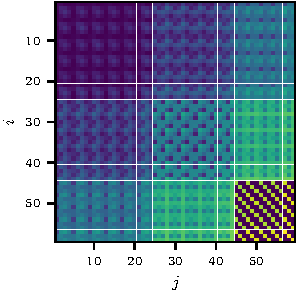
\includegraphics[width=1.0\linewidth]{../kfs/plots/synthetic_cvec_ggn_full.pdf}
  \end{minipage}
  \hfill
  \begin{minipage}[t]{0.485\linewidth}
    \centering
    GGN ($\cvec$)\vspace{1ex}
    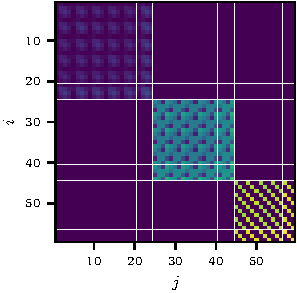
\includegraphics[width=1.0\linewidth]{../kfs/plots/synthetic_cvec_ggn_kfac.pdf}
  \end{minipage}
  \\
  \begin{minipage}[t]{0.485\linewidth}
    \centering
    MC-Fisher ($\cvec$)\vspace{1ex}
    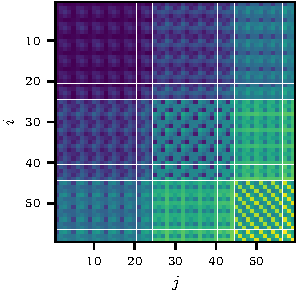
\includegraphics[width=1.0\linewidth]{../kfs/plots/synthetic_cvec_mcfisher_100_full.pdf}
  \end{minipage}
  \hfill
  \begin{minipage}[t]{0.485\linewidth}
    \centering
    MC-Fisher ($\cvec$)\vspace{1ex}
    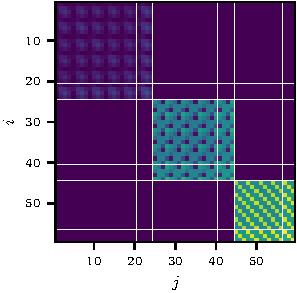
\includegraphics[width=1.0\linewidth]{../kfs/plots/synthetic_cvec_mcfisher_100_kfac.pdf}
  \end{minipage}
  \\
  \begin{minipage}[t]{0.485\linewidth}
    \centering
    Emp-Fisher ($\cvec$)\vspace{1ex}
    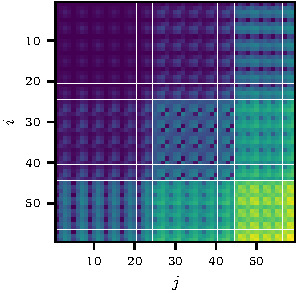
\includegraphics[width=1.0\linewidth]{../kfs/plots/synthetic_cvec_empfisher_full.pdf}
  \end{minipage}
  \hfill
  \begin{minipage}[t]{0.485\linewidth}
    \centering
    Emp-Fisher ($\cvec$)\vspace{1ex}
    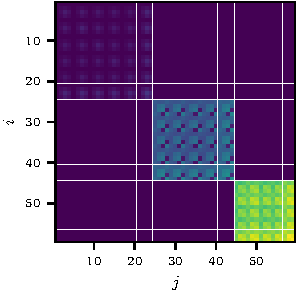
\includegraphics[width=1.0\linewidth]{../kfs/plots/synthetic_cvec_empfisher_kfac.pdf}
  \end{minipage}
  \caption{\textbf{Full curvatures and their corresponding KFAC approximation using $\cvec$-flattening}.
    All curvatures were evaluated on synthetic data ($N = 100$) using an MLP with three fully-connected layers and ReLU activations (5-4-4-3) and square loss.
    For the MC-sampled Fisher, we consider $M = 100$ samples.
    This follows the setup in \Cref{fig:hessian-block-structure}.
    KFAC concatenates the weight and bias of each layer.
    Produced with \repofile{plots/synthetic_kfac}.}
  \label{fig:cvec-kfac-full-comparison}
\end{figure}
\switchcolumn[0]

Building on the scaffold and code from the previous chapter, we now introduce, implement, and test the KFAC approximation for the weights (or combined weights and bias) of fully-connected layers (\texttt{torch.nn.Linear}).
See \Cref{fig:rvec-kfac-full-comparison,fig:cvec-kfac-full-comparison} for visualizations.

Our discussion will primarily center on regression settings with deep linear networks---MLPs composed of dense layers without nonlinearities.
This setting provides an ideal framework for understanding the core approximations behind KFAC and verifying them numerically through rigorous testing.
We focus on the formulation from \citet{martens2015optimizing}, which was originally introduced for standard MLP architectures, where linear layers do not exhibit weight sharing.

Other layers, like convolutions and linear layers inside the attention mechanism, exhibit weight sharing.
We deliberately exclude these aspects here and focus on linear layers without weight sharing.
Future versions of this tutorial may include them.

\switchcolumn[1]
\begin{figure}[!h]
  \centering
  \begin{minipage}[t]{0.485\linewidth}
    \centering
    \textbf{Full}
  \end{minipage}
  \hfill
  \begin{minipage}[t]{0.485\linewidth}
    \centering
    \textbf{KFAC}
  \end{minipage}
  \\
  \begin{minipage}[t]{0.485\linewidth}
    \centering
    GGN ($\rvec$)\vspace{1ex}
    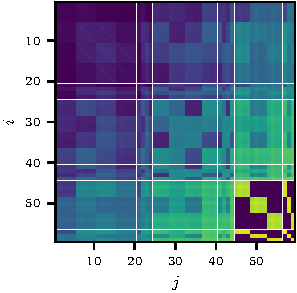
\includegraphics[width=\linewidth]{../kfs/plots/synthetic_rvec_ggn_full.pdf}
  \end{minipage}
  \hfill
  \begin{minipage}[t]{0.485\linewidth}
    \centering
    GGN ($\rvec$)\vspace{1ex}
    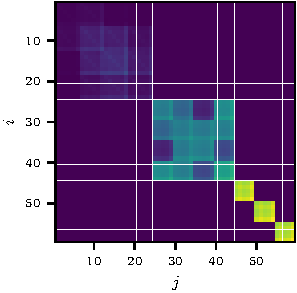
\includegraphics[width=\linewidth]{../kfs/plots/synthetic_rvec_ggn_kfac.pdf}
  \end{minipage}
  \\
  \begin{minipage}[t]{0.485\linewidth}
    \centering
    MC-Fisher ($\rvec$)\vspace{1ex}
    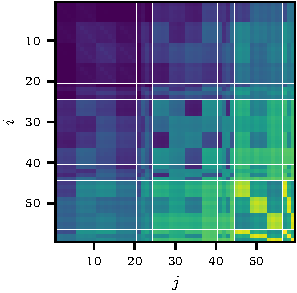
\includegraphics[width=\linewidth]{../kfs/plots/synthetic_rvec_mcfisher_100_full.pdf}
  \end{minipage}
  \hfill
  \begin{minipage}[t]{0.485\linewidth}
    \centering
    MC-Fisher ($\rvec$)\vspace{1ex}
    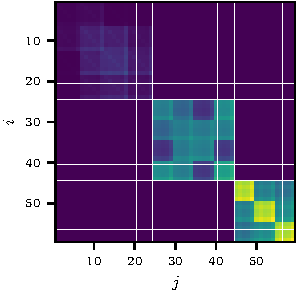
\includegraphics[width=\linewidth]{../kfs/plots/synthetic_rvec_mcfisher_100_kfac.pdf}
  \end{minipage}
  \\
  \begin{minipage}[t]{0.485\linewidth}
    \centering
    Emp-Fisher ($\rvec$)\vspace{1ex}
    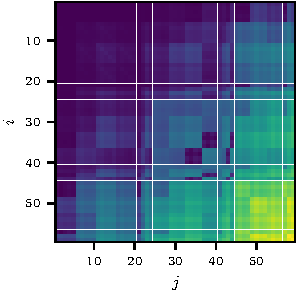
\includegraphics[width=\linewidth]{../kfs/plots/synthetic_rvec_empfisher_full.pdf}
  \end{minipage}
  \hfill
  \begin{minipage}[t]{0.485\linewidth}
    \centering
    Emp-Fisher ($\rvec$)\vspace{1ex}
    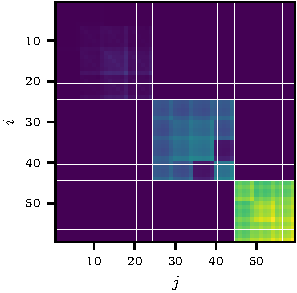
\includegraphics[width=\linewidth]{../kfs/plots/synthetic_rvec_empfisher_kfac.pdf}
  \end{minipage}
  \caption{\textbf{Full curvatures and their corresponding KFAC approximation using $\rvec$-flattening.}
    All curvatures were evaluated on synthetic data ($N = 100$) using an MLP with three fully-connected layers and ReLU activations (5-4-4-3) and square loss.
    For the MC-sampled Fisher, we consider $M = 100$ Monte Carlo samples.
    This follows the setup in \Cref{fig:hessian-block-structure}.
    KFAC concatenates the weight and bias of each layer.
    Produced with \repofile{plots/synthetic_kfac}.}
  \label{fig:rvec-kfac-full-comparison}
\end{figure}

\switchcolumn[0]

Let's formalize the layer whose curvature we approximate with KFAC in this chapter:

\begin{setup}[Linear layer inside a neural net]\label{setup:linear_layer}
  Consider a linear layer with weights $\mW \in \sR^{D_{\text{out}}\times D_{\text{in}}}$ and bias $\vb \in \sR^{D_{\text{out}}}$ in a neural net $f(\cdot, \vtheta)$.
  The network's prediction feeds into a criterion function, and we compute an empirical risk over a dataset of $N$ points, incorporating a reduction factor $R$.
  Our goal is to approximate the curvature matrix block $\mC(\vec \mW)$.

  For each datum $n$, the layer processes an input vector $\vx_n \in \sR^{D_{\text{in}}}$, producing an output vector $\vz_{n} \in \sR^{D_{\text{out}}}$ as follows
  $$ \vz_{n} = \mW \vx_{n} + \vb\,.$$
  Denote the network's prediction for datum $n$ by $\vf_n \in \sR^{\dim(\gF)}$.
  For each backprograted vector $\blacktriangle_{n,c} \in \sR^{\dim(\gF)}$, we denote the layer's output gradient as
  $$\vg_{n,c} = (\jac_{\vz_{n}} \vf_n)^{\top} \blacktriangle_{n,c} \in \sR^{D_{\text{out}}}\,.$$

  We will often neglect the bias and focus on approximating the curvature for the weight matrix $\mW$ alone.
  The bias can always be incorporated into the weight matrix by concatenation into a single weight matrix $\tilde{\mW}$ and by augmenting the input vectors with an additional constant:
  \begin{align*}
    \tilde{\mW} &= \begin{pmatrix} \mW & \vb \end{pmatrix} \in \sR^{D_{\text{out}} \times (D_{\text{in}} + 1)}\,, \\
    \tilde{\vx} &= \begin{pmatrix} \vx \\ 1 \end{pmatrix} \in \sR^{D_{\text{in}} + 1}\,.
  \end{align*}
  Thus, the derivations below hold equivalently for $\tilde{\mW}, \tilde{\vx}$ in place of $\mW, \vx$.
\end{setup}


% \begin{caveat}
%   In many modern neural networks, a linear layer processes a sequence of $S$ input vectors, transforming $(\vx_{n,1}, \dots, \vx_{n, S})$ into corresponding outputs $(\vz_{n, 1}, \dots, \vz_{n, S})$.
%   This is known as a linear layer with \emph{weight sharing}, and a key distinction arises depending on whether the layer processes each sequence element independently or not.
%   \begin{itemize}
%   \item \textbf{Independent processing:} The sequence dimension $S$ can be merged with the batch dimension $N$, effectively treating the inputs as a larger batch.
%   \item \textbf{Non-independent processing:} In cases like convolutional layers with additional pooling, the sequence elements interact, and special handling is required.
%   \end{itemize}

%   For a more detailed discussion on challenges associated with general weight-sharing, see~\citet{eschenhagen2023kroneckerfactored}.
% \end{caveat}


\subsection{Derivation of KFAC}

We now derive the KFAC approximation for a linear layer with weights $\mW$, input vector $\vx$, and output vector $\vz = \mW\vx$ (\Cref{setup:linear_layer}).
Following convention in the literature, we assume column-major ($\cvec$) flattening.

\paragraph{Exact curvature matrix.}
Recall from \Cref{eq:common-structure} that the curvature matrix \wrt $\mW$ takes the form
\begin{align*}
  &\mC(\cvec \mW) \\
  &\begin{aligned}=
    R \sum_n \sum_c &(\jac^{\cvec}_{\mW}\vz_n)^{\top} \\
                    &(\jac^{\cvec}_{\vz_n}\vf_n)^{\top}
                      \blacktriangle_{n,c} \blacktriangle_{n,c}^{\top}
                      (\jac^{\cvec}_{\vz_n}\vf_n) \\
                    &(\jac^{\cvec}_{\mW}\vz_n)\,.
  \end{aligned}
\end{align*}
We recall from \Cref{ex:linear_layer_jacobians} that the Jacobian of a linear layer's output \wrt its weights is
$$ \jac^{\cvec}_{\mW}\vz_n = \vx_n^{\top} \otimes \mI_{D_{\text{out}}}\, $$
where $\vx_n \in \R^{D_\text{in}}$ is the layer's input.
With that, and using the Kronecker product properties from \Cref{sec:mem_comp_eff_kron}, we see that the curvature matrix is a sum of Kronecker products:
\begin{align*}
  &\mC(\cvec \mW)
  \\
  &\begin{aligned}
    = R \sum_n \sum_c &(\vx_n \otimes \mI_{D_{\text{out}}}) \vg_{n,c} \\
                      & \vg_{n,c}^{\top} (\vx_n^{\top} \otimes \mI_{D_{\text{out}}})
  \end{aligned}\\
  &\begin{aligned}
    = R \sum_n \sum_c &(\vx_n \otimes \mI_{D_{\text{out}}}) \vg_{n,c} \\
                      &\left[(\vx_n \otimes \mI_{D_{\text{out}}}) \vg_{n,c} \right]^{\top}
  \end{aligned}\\
  &\begin{aligned}
    = R \sum_n \sum_c &\left( \vx_n \otimes \vg_{n,c} \right)\left( \vx_n \otimes \vg_{n,c} \right)^{\top}
  \end{aligned}\\
  &= R \sum_n \sum_c \left( \vx_n \otimes \vg_{n,c} \right)
    \left( \vx_n^{\top} \otimes \vg_{n,c}^{\top} \right) \\
  &= R \sum_n \sum_c \left(\vx_n \vx_n^{\top}\right) \otimes \left(\vg_{n,c} \vg_{n,c}^{\top}\right)\,.
\end{align*}

\switchcolumn[1]*
\begin{example}[Motivation for KFAC's expectation approximation]
  \label{ex:just_kfac_exp_approx}
  KFAC's expectation approximation can be derived from an optimality condition under specific assumptions to preserve a Kronecker structure.

  Consider the curvature matrix
  \begin{align*}
    \mC
    &=
      \textstyle
      R \sum_{n=1}^N
      (\vx_n \otimes \mI_{D_{\text{out}}})
      \vg_n \vg_n^{\top}
      (\vx_n^{\top} \otimes \mI_{D_{\text{out}}})\,.
  \end{align*}
  Our goal is to approximate $\mC$ with a single Kronecker product.

  To make this expression more compact, stack the vectors $\vx_n$ and $\vg_n$ into matrices:
  \begin{align*}
    \mX
    &=
      \begin{pmatrix}
        \vx_1 & \vx_2 & \ldots & \vx_N
      \end{pmatrix}
      \in \sR^{D_{\text{in}} \times N}\,,
    \\
    \mG
    &=
      \begin{pmatrix}
        \vg_1 & \vg_2 & \ldots & \vg_N
      \end{pmatrix}
      \in \sR^{D_{\text{out}} \times N}\,.
  \end{align*}
  and rewrite $\mC$ in terms of these matrices:
  \begin{align*}
    \mC = R (\mX \otimes \mI_{D_{\text{out}}}) \cvec(\mG) \cvec(\mG)^{\top}(\mX^{\top} \otimes \mI_{D_{\text{out}}}).
  \end{align*}
  Looking at this expression, we realize that an easy way to achieve a single Kronecker product is to approximate $\cvec(\mG) \cvec(\mG)^{\top} \approx \mI_{D_{\text{in}}} \otimes \mB$ with $\mB \in \sR^{D_{\text{out}}\times D_{\text{out}}}$.
  Then we would have
  \begin{align*}
    \mC
    &\approx
      R (\mX \otimes \mI_{D_{\text{out}}})
      (\mI_{D_{\text{in}}} \otimes \mB)
      (\mX^{\top} \otimes \mI_{D_{\text{out}}})
    \\
    &=
      R \mX \mX^{\top} \otimes \mB
      =
      \textstyle
      R \left(\sum_{n=1}^N \vx_n \vx_n^{\top}\right) \otimes \mB\,.
  \end{align*}
  To obtain $\mB$, we minimize the squared Frobenius norm residual:
  \begin{align*}
    \begin{split}
      &\argmin_{\mB}
        \left\lVert
        \cvec(\mG) \cvec(\mG)^{\top} - \mI_{D_{\text{in}}} \otimes \mB
        \right\rVert_2^2.
    \end{split}
    \intertext{Expanding the Kronecker structure, this is equivalent to}
    \begin{split}
      &\argmin_{\mB}
        \left\lVert
        \begin{pmatrix}
          \vg_1 \vg_1^{\top} -\mB & \dots & \vg_1 \vg_N^{\top} \\
          \vdots & \ddots & \vdots \\
          \vg_N \vg_1^{\top} & \dots & \vg_N \vg_N^{\top} - \mB \\
        \end{pmatrix}
        \right\rVert_2^2
      \\
      &=
        \argmin_{\mB}
        \left\lVert
        \begin{pmatrix}
          \vg_1 \vg_1^{\top} - \mB & \dots & \vzero \\
          \vdots & \ddots & \vdots \\
          \vzero & \hdots & \vg_N \vg_N^{\top} - \mB \\
        \end{pmatrix}
        \right\rVert_2^2
      \\
      &=
        \argmin_{\mB}
        \sum_{n=1}^N
        \left\lVert
        \vg_n \vg_n^{\top} - \mB
        \right\rVert_2^2
      \\
      &=
        \argmin_{\mB}
        \sum_{n=1}^N
        \sum_{i,j = 1}^{D_{\text{out}}}
        \left(
        [\vg_n]_i [\vg_n]_j - [\mB]_{i,j}
        \right)^2 \,.
    \end{split}
  \end{align*}
  Taking the derivative \wrt $\mB$ and setting it to zero yields for all $k, l \in \{1, \dots, D_{\text{out}}\}$,
  \begin{align*}
    &\frac{\partial \left(
      \sum_{n=1}^N
      \sum_{i,j = 1}^{D_{\text{out}}}
      \left(
      [\vg_n]_i [\vg_n]_j - [\mB]_{i,j}
      \right)^2
      \right)
      }{
      \partial [\mB]_{k,l}
      }
    \\
    &=
      2 \sum_{n=1}^N
      \left(
      [\mB]_{k,l} -  [\vg_n]_k [\vg_n]_l
      \right)
    \\
    &=
      2 \left( N[\mB]_{k,l} - \sum_{n=1}^N [\vg_n]_k [\vg_n]_l \right)
      \stackrel{!}{=} 0
    \\
    &\implies
      \mB = \frac{1}{N} \sum_{n=1}^N \vg_n \vg_n^{\top}
      = \frac{1}{N} \mG \mG^{\top}.
  \end{align*}
  Thus, under this optimality condition, the best choice for $\mB$ is the empirical covariance of the gradient vectors:
  \begin{align*}
    \mC
    \approx
    \left(R \sum_n \vx_n \vx_n^\top \right)
    \otimes
    \left(\frac{1}{N} \sum_{n'} \vg_{n'} \vg_{n'}^\top \right).
  \end{align*}
  This is precisely the expectation approximation used in KFAC.
\end{example}
\switchcolumn[0]

\paragraph{From sum of Kronecker products to single Kronecker product.}
The last step is to approximate the sum of Kronecker products by a single Kronecker product.
To do that, we use the so-called KFAC's expectation approximation (see \Cref{ex:just_kfac_exp_approx} for further motivation):

\begin{definition}[KFAC's expectation approximation]
  \label{def:kfac_exp_approx}
  Consider two sets of $N$ vectors $\{\vx_{n}\}_{n=1}^N$ and $\{\vg_{n}\}_{n=1}^N$ where each $\vx_n$ is input-based and each $\vg_n$ is output-gradient-based.
  KFAC approximates the sum of Kronecker products of their self-outer products by a single Kronecker product, using the following expectation approximation:
  \begin{subequations}\label{eq:expectation_approximation}
    \begin{align}
      \begin{split}
        &\sum_{n=1}^{\textcolor{VectorOrange}{N}} \vx_n\vx_n^{\top} \otimes \vg_n \vg_n^{\top}
        \\
        &\qquad\approx
          \left( \sum_{n=1}^N \vx_n \vx_n^{\top} \right)
          \otimes
          \frac{
          \left( \textcolor{VectorOrange}{\sum_n} \vg_n \vg_n^{\top} \right)
          }{\textcolor{VectorOrange}{N}}.
      \end{split}
      \intertext{In words, we sum the outer products on the left and right of the Kronecker product independently and divide by the number of outer products in the term containing the gradient vectors.
      In expectation notation (expectation meaning averaging over all values of $n$, \ie $\E_n[\bullet_n] = \nicefrac{1}{N} \sum_{n=1}^N \bullet_n$), we can write this approximation more conveniently as}
      \begin{split}
        &\E_n \left[ \vx_n \vx_n^{\top} \otimes \vg_n \vg_n^{\top} \right]
        \\
        &\qquad\approx N
          \E_n \left[ \vx_n \vx_n^{\top} \right]
          \otimes
          \E_n \left[ \vg_n \vg_n^{\top} \right]\,,
      \end{split}
    \end{align}
  \end{subequations}
  \ie `pull' the expectation into the Kronecker factors.
\end{definition}

Applying \Cref{def:kfac_exp_approx}, we obtain the curvature matrix's KFAC approximation:
\begin{align*}
  \mC&(\cvec \mW) \\
  \approx&
           \underbrace{\left( R \sum_n \vx_n \vx_n^{\top} \right)}_{\text{input-based}}
           \otimes
           \underbrace{\left( \frac{1}{N} \sum_n \sum_c \vg_{n,c} \vg_{n,c}^{\top} \right)}_{\text{grad-output-based}}
  \\
  =& \kfac(\mC(\cvec \mW))\,.
\end{align*}

\paragraph{Changing flattening swaps the Kronecker factors.}
Had we done the same derivation using the $\rvec$-flattening scheme where the output-parameter Jacobian takes the form (\Cref{ex:linear_layer_jacobians})
$$ \jac^{\rvec}_{\mW}\vz_n = \mI_{D_{\text{out}}} \otimes \vx_n^{\top}\,,$$
we would have found the order of Kronecker factors to reverse,
\begin{align*}
  \mC&(\rvec \mW) \\
  \approx&
           \left( \frac{1}{N} \sum_n \sum_c \vg_{n,c} \vg_{n,c}^{\top} \right)
           \otimes
           \left( R \sum_n \vx_n \vx_n^{\top} \right)
  \\
  =& \kfac(\mC(\rvec \mW))\,.
\end{align*}
This is important to keep in mind for KFAC implementations, as libraries like PyTorch use $\rvec$-flattening.
In summary, we have the following:

\switchcolumn[1]
\codeblock{kfac/expand_Linear}
\switchcolumn[0]

\begin{definition}[KFAC for a linear layer without weight sharing, \Cref{kfac/expand_Linear}]\label{def:kfac_expand_linear}
  Consider a linear layer inside a neural network from \Cref{setup:linear_layer}.
  The \emph{KFAC approximation} of a curvature matrix \wrt the layer's weights is given by
  \begin{subequations}\label{eq:kfac_expand_linear}
    \begin{align}
      \begin{split}
        &\kfac(\vec \mW) \approx \mC(\vec \mW)
        \\
        &\quad=
          \begin{cases}
            \mA \otimes \mB & \vec = \cvec
            \\
            \mB \otimes \mA & \vec = \rvec
          \end{cases}\,,
      \end{split}
    \end{align}
    with the input-based factor
    \begin{align}
      \mA &= R \sum_{n=1}^N \vx_{n} \vx_{n}^{\top}\in \sR^{D_{\text{in}} \times D_{\text{in}}}
                        \intertext{and the output-gradient-based factor}
                        \mB &= \frac{1}{N}\sum_{n=1}^N \sum_c \vg_{n,c} \vg_{n,c}^{\top}\in \sR^{D_{\text{out}} \times D_{\text{out}}}
    \end{align}
  \end{subequations}
  and $\vg_{n,c}$ the backpropagated vector of a curvature matrix at layer output $\vz$ given by $$\vg_{n,c} = (\jac_{\vz_{n,s}}^{\vec}\vf_n)^{\top} \blacktriangle_{n,c}\,.$$
\end{definition}

% NOTE This part is about weight sharing, which will not be in the first version.
\begin{comment}
  Similarly, we can justify flattening an additional sequence dimension into the batch dimension when no additional reduction occurs along any axes in the neural network.

  To see this, consider a sequence of input vectors represented as a matrix-valued input
  \begin{align*}
    \mX_n = (\vx_{n, 1}, \dots, \vx_{n, s}),
  \end{align*}
  where $S$ is the sequence length.
  The corresponding sequence of output vectors is given by:
  \begin{align*}
    \mZ_n = \left( \vz_{n, 1}, \dots, \vz_{n,s} \right),
  \end{align*}
  and the backpropagated vectors, regardless of their specific type, are stored in the matrix
  \begin{align*}
    \mG_{n, c} = (\vg_{n, c, 1}, \dots, \vg_{n, c, s}).
  \end{align*}
  Then, the curvature matrix takes the form:
  \begin{align*}
    \mC(&\cvec \mW) \\
        &\begin{aligned}
          =R\sum_n \sum_c \sum_s
          &(\jac^{\cvec}_{\mW}\vz_{n,s})^{\top} \\
          &\cvec\vg_{n,c,s} (\cvec\vg_{n,c,s})^{\top} \\
          &\jac^{\cvec}_{\mW}\vg_{n,c,s}
        \end{aligned}\\
        &\begin{aligned}
          = R \sum_n \sum_c &(\mX_n \otimes \mI_{\vz_n}) \\
                            &\cvec \mG_{n,c}(\cvec \mG_{n,c})^{\top} \\
                            &(\mX_n^{\top} \otimes \mI_{\vz_n}).
        \end{aligned}
  \end{align*}
  A key observation is that the matrix $\vec\mG_{n,c} (\vec\mG_{n,c})^{\top}$ has dimensions $S D_{\text{out}} \times S D_{\text{out}}$ and does not simplify into a single Kronecker product.

  Similar to Example~\ref{ex:just_kfac_exp_approx}, we would like to find an approximation
  \begin{align*}
    \cvec\mG_{n,c} (\cvec\mG_{n,c})^{\top} \approx \mK \otimes \mI_{D_\text{out}}
  \end{align*}
  to simplify the expression into a single Kronecker structure.

  Using the same optimality condition and arguments, it is straightforward to show that:
  \begin{align*}
    \argmin_{\mK}
    &\left\lVert
      \cvec \mG_{n,c} (\cvec \mG_{n,c})^{\top} - \mK \otimes \mI_{D_{\text{out}}}
      \right\rVert_2 \\
    &=
      \frac{1}{S} \mG_{n,c} \mG_{n,c}^{\top}.
  \end{align*}
  This result tells us that the optimal Kronecker approximation is again obtained by averaging the diagonal blocks of size $S\times S$, simplifying the curvature matrix to:
  \begin{align*}
    \mC(\cvec\mW)
    &\approx
      R \sum_n \sum_c
      \mZ_n \mZ_n^{\top} \otimes \frac{1}{S} \mG_{n,c} \mG_{n,c}^{\top}
    \\
    &= R \sum_n \sum_s \vz_{n,s} \vz_{n,s}^{\top} \\
    &\quad\otimes \sum_{s'} \sum_c \frac{1}{S} \vg_{n,s',c} \vg_{n,s',c}^{\top}
      \intertext{Applying KFAC's expectation approximation from \Cref{def:kfac_exp_approx}, we obtain}
    &\approx
      \left(R \sum_n \sum_s \vz_{n,s} \vz_{n,s}^{\top}\right)
    \\
    &\quad\otimes \left( \frac{\textcolor{VectorOrange}{\sum_n} \textcolor{VectorTeal}{\sum_s}\sum_c \vg_{n,s,c} \vg_{n,s,c}^{\top}}{\textcolor{VectorOrange}{N} \textcolor{VectorTeal}{S}} \right).
  \end{align*}
  This equation highlights that the sequence dimension (highlighted in \textcolor{VectorTeal}{teal}) is treated exactly like the batch dimension (highlighted in \textcolor{VectorOrange}{orange}) in KFAC's expectation approximation.
  Consequently, if no additional reduction occurs along the sequence dimension, it can be flattened into the batch dimension without affecting the approximation structure.
\end{comment}

\subsection{Tests}

To verify our KFAC implementation, we need tests.
This raises an important question: When does the approximation in \Cref{eq:expectation_approximation} become exact?
In general, KFAC's expectation approximation becomes exact whenever one of $\{\vx_n\}_n$ or $\{\vg_{n,c}\}_{n,c}$ is data-independent, \ie, does not depend on $n$.
There are two notable cases where this happens, one of which is relatively obvious.

\switchcolumn[1]
\codeblock{kfac_tests/mlp_batch_size_1}
\switchcolumn[0]

\subsubsection{Data Set Size 1}
A particularly straightforward case occurs when summation over $n$ disappears, \ie when the dataset is only a single data point or $N$ identical data points.
Hence, we have the following

\begin{test}[KFAC for linear layers in an MLP with one data point, \Cref{kfac_tests/mlp_batch_size_1}]\label{test:kfac_expand_linear_no_weight_sharing_batch_size_1}
  Consider a multi-layer perceptron (MLP)
  \begin{align*}
    f = \phi^{(L)} \circ f^{(L)} \circ \ldots \circ \phi^{(1)} \circ f^{(1)}\,.
  \end{align*}
  Each layer consists of a dense (linear) transformation $f^{(l)}$ (satisfying \Cref{setup:linear_layer}) followed by a pointwise activation $\phi^{(l)}$.
  Let $\mW^{(l)}$, $\vb^{(l)}$, and $\tilde{\mW}^{(l)} = \begin{pmatrix} \mW^{(l)} & \vb^{(l)} \end{pmatrix}$ denote the weight, bias, and concatenated parameters of the dense layer $l$.

  Now, assume that the dataset consists of only one data point, $\sD = \{ (\vx, \vy) \}$, and we have a criterion function $c = - \log r$, which can be interpreted as negative log-likelihood.

  Then, KFAC becomes exact for all layers $l = 1, \dots, L$ and any flattening scheme $\vec$ in the following sense:
  \begin{itemize}[leftmargin=0.5cm]
  \item KFAC-type-II equals the GGN
    \begin{align*}
      \kfac(\mG(\vec \tilde{\mW}^{(l)})) = \mG(\vec \tilde{\mW}^{(l)})
    \end{align*}
  \item KFAC-MC converges to the GGN
    \begin{align*}
      \lim_{M \to \infty} &\kfac(\mF^{\text{I}}(\vec\tilde{\mW}^{(l)}))
      \\
                          &= \mG(\vec \tilde{\mW}^{(l)})
    \end{align*}
  \item KFAC-empirical coincides with the empirical Fisher
    \begin{align*}
      \kfac(\mE(\vec\tilde{\mW}^{(l)})) = \mE(\vec \tilde{\mW}^{(l)})
    \end{align*}
  \end{itemize}
\end{test}

This test serves as a basic functionality check for KFAC, particularly regarding the criterion function and its backpropagated vectors $\blacktriangle_{n,c}$.

\switchcolumn[1]
\codeblock{kfac_tests/deep_linear_regression}
\switchcolumn[0]

\subsubsection{Regression with Deep Linear Nets}

A more subtle and interesting case where the KFAC approximation becomes exact is for deep linear networks with square loss.
In this setting, the backpropagated vectors $\vg_{n,c}$ become independent of $n$ because the network's prediction is linear \wrt each layer's parameter $\mW^{(l)}$ (but not linear \wrt the \emph{full} parameter vector $\vtheta$).

Recall that $\vg_{n,c}$ depends on the backpropagated vector $\blacktriangle_{n,c}$ and the Jacobian of the prediction \wrt the layer's output $\jac_{\vz_n} \vf_n$.
For a square loss function, $\blacktriangle_{n,c}$ is often independent of $n$:
\begin{itemize}
\item In type-II Fisher, it corresponds to a column of the identity matrix.
\item In Monte Carlo (MC) Fisher, it is simply a normally distributed random number.
\end{itemize}
Further, if all layers in the net are linear, then all prediction-intermediate Jacobians remain constant and independent of $n$.
Thus, in this setting, the KFAC approximation becomes exact in the limit, as originally found by \citet{bernacchia2018exact}.

\begin{test}[KFAC for regression with a deep linear net (no nonlinear layers), \Cref{kfac_tests/deep_linear_regression}]
  Consider a deep linear network consisting of $L$ fully-connected layers
  \begin{align*}
    f = f^{(L)} \circ f^{(L-1)} \circ \ldots \circ f^{(1)}
  \end{align*}
  with weights $\mW^{(l)}$, bias $\vb^{(l)}$, and concatenated parameters $\tilde{\mW}^{(l)} = \begin{pmatrix} \mW^{(l)} & \vb^{(l)} \end{pmatrix}$.
  Assume the network processes a vector-valued input per datum and performs regression with square loss on an arbitrary dataset $\sD = \{ (\vx_n, \vy_n) \mid n = 1, \dots, N \}$.
  Then, for each layer $l=1,\dots,L$ and any chosen flattening scheme $\vec$, the following identities hold:
  \begin{itemize}[leftmargin=0.5cm]
  \item KFAC-type-II equals the GGN
    \begin{align*}
      \kfac(\mG(\vec \tilde{\mW}^{(l)}))
      =
      \mG(\vec\tilde{\mW}^{(l)})
    \end{align*}
  \item KFAC-MC converges to the GGN
    \begin{align*}
      \lim_{M \to \infty}& \kfac(\mF^{\text{I}}(\vec \tilde{\mW}^{(l)}))
      \\&=
      \mG(\vec \tilde{\mW}^{(l)})
    \end{align*}

  \end{itemize}
  However, KFAC-empirical \emph{differs} from the empirical Fisher,
  \begin{align*}
    \kfac(\mE(\vec \tilde{\mW}^{(l)}))
    \neq
    \mE(\vec \tilde{\mW}^{(l)})\,,
  \end{align*}
  as the backpropagated vector $\blacktriangle_{n,c}$ depends on $\vf_n$ and therefore remains dependent on $n$.
\end{test}

This test is useful for preventing scaling bugs in the Kronecker factor computations.
Additionally, it remains valid when incorporating an independent sequence dimension $S$, \ie in the presence of weight sharing, provided that the network treats sequence elements independently.
Although weight sharing is not of our interest in this chapter, we have already included such a slightly more general test case in \Cref{kfac_tests/deep_linear_regression}.

%%% Local Variables:
%%% mode: latex
%%% TeX-master: "../main"
%%% End:


  % \section{KFAC for Convolution Layers}
  % The goal of this section should be to describe the KFAC approximation from.

  % \switchcolumn[1]*
  % \codeblock{kfac/expand_ConvNd}
  % \switchcolumn[0]

  % \switchcolumn[1]*
  % \codeblock{kfac/reduce_ConvNd}
  % \switchcolumn[0]

  % \switchcolumn[1]*
  % \codeblock{kfac_tests/reduce_shallow_cnn}
  % \switchcolumn[0]
\end{paracol}

\clearpage

\begin{paracol}{1}
  \section{Cheatsheet: KFAC}
  \begin{itemize}
  \item General KFAC Scaffold
  \begin{align*}
    \mC(\vtheta^{(i)})
    \approx
    \kfac(\mC(\vtheta^{(i)}))
    \coloneqq \mA^{(i)} \otimes \mB^{(i)}
  \end{align*}
  with
  \begin{itemize} 
    \item $\mC(\vtheta^{(i)})
    = R \sum_n
    (\jac_{\vtheta^{(i)}} \vf_n)^{\top}
    \left[ \bullet(\vf_n, \vy_n) \right]
    (\jac_{\vtheta^{(i)}} \vf_n)$
    \item $\bullet(\vf_n, \vy_n) = \sum_{c=1}^{\dim(\gF)} \blacktriangle_c(\vf_n, \vy_n) (\blacktriangle_c(\vf_n, \vy_n))^{\top}$ \quad (which together with $R$ depends on the curvature target)
    \item $\mA^{(i)} = \mA^{(i)}( \{\vx_{n}^{(i-1)}\}_n )$ \quad (input-based factor)
    \item $\mB^{(i)} = \mB^{(i)}( \{ (\jac_{\vx_n^{(i)}}\vf_{n})^{\top} \blacktriangle_{n,c}\}_{n,c})$ \quad (output-gradient-based factor)
  \end{itemize}
  \item Backpropagated vectors $\{ \blacktriangle_{n,c} \}_{n,c}$
    \begin{itemize}
    \item Type-II: $\blacktriangle_{n,c} = [\mS_n]_{:,c}$ for $c = 1, \dots, C$ where $\mS_n \mS_n^{\top} = \hess_{\vf_n} c(\vf_n, \vy_n)$
      \begin{itemize}
      \item Square loss: $\blacktriangle_{n,c} = [\mI]_{n,c}$  (one-hot vector, does not depend on $n$)
      \item Softmax cross-entropy loss: $\blacktriangle_{n,c} =  \sqrt{[\softmax(\vf_n)]_c} (\onehot(c) - \softmax(\vf_n))$
      \end{itemize}

    \item MC: $\blacktriangle_{n,m} = - \nabla_{\vf_n} \log r(\rvy = \tilde{\vy}_{n,m} \mid \rvf = \vf_n)$ where $\tilde{\vy}_{n,m} \stackrel{\text{i.i.d.}}{\sim} r(\rvy \mid \rvf = \vf_n)$
      \begin{itemize}
      \item Square loss: $\blacktriangle_{n,m} = \tilde{\vy}_{n,m} - \vf_n$ where $\vy_{n,m} \stackrel{\text{i.i.d.}}{\sim} \gN(\rvy \mid \vmu = \vf_n, \mSigma = \mI)$\\
        $\Leftrightarrow \blacktriangle_{n,m} = \tilde{\vy}$ where $\tilde{\vy} \stackrel{\text{i.i.d.}}{\sim} \gN(\rvy \mid \mu = \vzero, \mSigma = \mI)$ (does not depend on $n$)
        \item Softmax cross-entropy loss
      \end{itemize}

    \item Empirical: $\blacktriangle_{n,1} = - \nabla_{\vf_n} \log r(\rvy = \vy_n \mid \rvf = \vf_n)$
      \begin{itemize}
      \item Square loss: $\blacktriangle_{n,1} = \vy_n - \vf_n$
      \item Softmax cross-entropy loss: $\blacktriangle_{n,1} = \softmax(\vf_n) - \onehot(y_n)$
      \end{itemize}
    \end{itemize}
  \item KFAC-expand for a linear layer
    \begin{align*}
      &\kfac_{\text{exp}}(\vec \mW) \approx \mC(\vec \mW)
      =
        \begin{cases}
          \mA_{\text{exp}} \otimes \mB_{\text{exp}} & \vec = \cvec
          \\
          \mB_{\text{exp}} \otimes \mA_{\text{exp}} & \vec = \rvec
        \end{cases}\,
    \end{align*}
    with
    \begin{align*} 
      \mA_{\text{exp}} = R \sum_{n=1}^N \vx_{n} \vx_{n}^{\top} \in \sR^{D_{\text{in}} \times D_{\text{in}}}, \qquad
      \mB_{\text{exp}} &= \frac{1}{N}\sum_{n=1}^N \sum_c \vg_{n,c} \vg_{n,c}^{\top}  \in \sR^{D_{\text{out}} \times D_{\text{out}}}
    \end{align*}
    where
    \begin{align*}
    \vg_{n,c} = (\jac_{\vz_{n,s}}^{\vec}\mF_n)^{\top} (\vec \blacktriangle_{n,c}).
    \end{align*}
  \item Test cases
    \begin{itemize}
      \item KFAC-expand for linear layers in an MLP (no weight sharing) and assuming a dataset with only a single data point:
        \begin{itemize}
          \item KFAC-expand-type-II coincides with the GGN, \ie,
            \begin{align*}
              \kfac^{\text{II}}_{\text{exp}}(\vec\tilde{\mW}^{(l)}) = \ggn^{\vec}_{\tilde{\mW}^{(l)}}\gL_{\sD}.
            \end{align*}
          \item KFAC-expand-MC converges to the GGN, \ie,
            \begin{align*}
              \lim_{M \to \infty} \kfac^{\text{MC}=M}_{\text{exp}}(\vec\tilde{\mW}^{(l)}) = \ggn^{\vec}_{\tilde{\mW}^{(l)}}\gL_{\sD}.
            \end{align*}
          \item KFAC-expand-empirical coincides with the Empirical Fisher (EF), \ie,
            \begin{align*}
              \kfac^{\text{E}}_{\text{exp}}(\vec\tilde{\mW}^{(l)}) = \ef^{\vec}_{\tilde{\mW}^{(l)}}\gL_{\sD}.
            \end{align*}
        \end{itemize}
      \item KFAC-expand for regression with a Deep Linear Network (no weight sharing and no nonlinear layers).
        \begin{itemize}
          \item KFAC-expand-type-II coincides with the GGN, \ie,
            \begin{align*}
              \kfac^{\text{II}}_{\text{exp}}(\vec \tilde{\mW}^{(l)}) = \ggn^{\vec}_{\tilde{\mW}^{(l)}} \gL_{\sD}\,.
            \end{align*}
          \item KFAC-expand-MC converges to the GGN as $M\rightarrow\infty$, \ie, 
            \begin{align*}
              \lim_{M \to \infty} \kfac^{\text{MC}=M}_{\text{exp}}(\vec \tilde{\mW}^{(l)}) = \ggn^{\vec}_{\tilde{\mW}^{(l)}} \gL_{\sD}\,.
            \end{align*}
          \item KFAC-expand-empirical does \emph{not} equal the empirical Fisher, \ie,
            \begin{align*}
              \kfac_{\text{exp}}^{\text{E}}(\vec \tilde{\mW}^{(l)})
              \neq
              \ef^{\vec}_{\tilde{\mW}^{(l)}} \gL_{\sD}\,.
            \end{align*}         
        \end{itemize}
      \end{itemize}
    \end{itemize}
%%% Local Variables:
%%% mode: latex
%%% TeX-master: "../main"
%%% End:

  \end{paracol}
\clearpage


\begin{paracol}{1}
  \section{Outlook}
  \paragraph{Summary.} In this manuscript, we provided a detailed overview of the seminal KFAC curvature approximation from the ground up, in both math and code.
In doing so, we first developed a collection of automatic differentiation utilities to access derivatives.
They play a crucial role in computing curvature information and help us make these concepts concrete for common operations used in deep learning, while serving as ground truth to verify our implementation.
Building on these fundamentals, we motivated using Kronecker products to approximate curvature matrices in neural networks, and introduced the KFAC approximation for linear layers in the absence of weight sharing, as originally described by \citet{martens2015optimizing}, showed how to apply it to different curvature matrices, and highlighted tests to verify its correctness.

\emph{We hope this tutorial is a helpful resource for both newcomers to the field who want to learn more about curvature matrices, their approximations, and common pitfalls, as well as experienced researchers who are seeking a pedagogical introduction and implementation they can use as a starting point to prototype their research idea.}

\paragraph{Call for contributions \& future work.} Although we believe that we covered the most essential aspects of KFAC, this tutorial does not address many important, albeit advanced, topics related to KFAC.
We invite anyone to contribute to this fully open-source effort (\href{\repourl}{\texttt{github.com/f-dangel/kfac-tutorial}}) to further improve the tutorial over time.
Specifically, we think the following ideas are promising to include in future versions:
\begin{itemize}
\item \textbf{Eigenvalue-corrected KFAC (EKFAC).}
  \citet{george2018fast} proposed the concept of eigenvalue correction to improve KFAC's approximation quality, and the resulting EKFAC has become the de facto standard for KFAC's application to training data attribution with influence functions~\cite{grosse2023studying,mlodozeniec2025influence}.
  The first step in computing EKFAC is to compute KFAC.
  In the second step, we only keep the space spanned by the Kronecker factors, and introduce a diagonal scaling term (the ``eigenvalues''), whose value is determined by minimizing the Frobenius norm residual between the original curvature matrix and the corrected KFAC approximation.
  This can be done cheaply.

\item \textbf{KFAC for linear layers with weight sharing.}
  We focused on explaining KFAC as introduced in the seminal paper by \citet{martens2015optimizing}, which considers multi-layer perceptrons where each layer processes a single vector per datum (\ie no weight sharing).
  However, modern neural networks like convolutional networks, transformers, or graph neural networks, process sequence-valued data and therefore naturally exhibit weight sharing across spatial or temporal dimensions.
  Depending on how the shared axis is treated when computing the loss, there exist two different KFAC approximations for linear layers with weight sharing, coined by \citet{eschenhagen2023kroneckerfactored}: KFAC-expand and KFAC-reduce.
  KFAC-reduce becomes relevant in scenarios where weight sharing occurs, and the shared dimension is explicitly reduced (\eg, summed or averaged) during the forward pass.
  Unlike KFAC-expand, which treats shared dimensions as independent by flattening them into a batch dimension, KFAC-reduce adjusts for this reduction by aggregating inputs and gradients across the shared dimension before forming Kronecker factors.
  The formalization of \citet{eschenhagen2023kroneckerfactored} allows KFAC to be extended to transformers, convolutional networks (containing the originally proposed method from \citet{grosse2016kroneckerfactored}), and graph neural networks.
  While we already introduced the \emph{expand} specifier in our implementation, we have not yet implemented the \emph{reduce} specifier and its related tests.

\item \textbf{Functional-style KFAC implementation.}
  One essential step for computing KFAC is accessing the inputs and outputs of layers.
  This is easy if the neural net consists entirely of \texttt{torch.nn.Module}s---and we assume this in our implementation---by using PyTorch's hook mechanism to intercept the forward pass and obtain the layer inputs (required for KFAC's input-based Kronecker factor) and outputs (required for KFAC's grad-output-based Kronecker factors).
  This is okay because most architectures used in practice are indeed implemented in a modular fashion.

  However, a functional-style implementation of KFAC, which had the ability to automatically trace and capture the inputs and outputs of linear operations inside a function representing the neural network (similar to KFAC's implementation in JAX \cite{botev2022kfac-jax}), would make KFAC accessible to libraries that adopt a functional style \citep[\eg][]{duffield2025scalable}.
  Such a more general approach is also helpful to incorporate more recent extensions of KFAC, for instance, to training Physics-informed neural networks \cite{dangel2024kroneckerfactored}, whose forward pass is done in Taylor mode arithmetic that differs from the standard forward pass and can therefore not be intercepted with module hooks.
  We believe that a functional-style implementation of KFAC in PyTorch can be achieved using the tracing mechanism of \texttt{torch.fx} \cite{reed2022torch}, which provides a modifiable presentation of the computation graph.
\end{itemize}

\subsection*{Acknowledgements}
We would like to thank Disen Liao for providing feedback on this manuscript.
Resources used in preparing this research were provided, in part, by the Province of Ontario, the Government of Canada through CIFAR, and companies sponsoring the Vector Institute.

%%% Local Variables:
%%% mode: LaTeX
%%% TeX-master: "../main"
%%% End:


\end{paracol}

\clearpage

\begin{paracol}{2}
  \section{Other aspects}
  \subsection{Weight tying, RNNs, PINNs}
  \subsection{Unnormalized densities}
  \subsection{KFAC for diffusion models}
\end{paracol}

\clearpage
{\footnotesize
  \bibliographystyle{icml2024.bst}
  \bibliography{references.bib}
}
%%% Local Variables:
%%% mode: latex
%%% TeX-master: "../main"
%%% End:


\appendix

\section{Important Loss Function Hessians and Their Symmetric Factorization}\label{app:loss_function_hessians}
TODO Write down the Hessian of BCEWithLogitsLoss.
%%% Local Variables:
%%% mode: latex
%%% TeX-master: "../main"
%%% End:


\end{document}

%%% Local Variables:
%%% mode: latex
%%% TeX-master: t
%%% End:
